 \setcounter{section}{0}% Change chapter counter
 \numberwithin{equation}{section}% Equation counter belongs to section
 \numberwithin{figure}{section}% Figure counter belongs to section
 \setcounter{chapter}{5}

\chapter{\texorpdfstring{Tree-level amplitudes}{6 Tree-level amplitudes}} \label{cha:6}
We now study string interactions . In this chapter, we will investigate the lowest-order amplitudes, which originate from surfaces with positive Euler number . We first describe the relevant Riemann surfaces and calculate the required CFT expectation values . Next, we will study scattering amplitudes, first for open strings and then for closed strings . Along the way, we will introduce an important generalization in open string theory: Chan-Paton factors . At the end of this section, we will return to CFT and discuss the general properties of expectation values .

\section{Riemann surfaces} \label{sec:6.1}

There are three types of Riemann surfaces with positive Euler number: the sphere, the disk, and the projective plane .

\subsection*{The Sphere}

\begin{figure}[!htbp]
	\begin{center}
		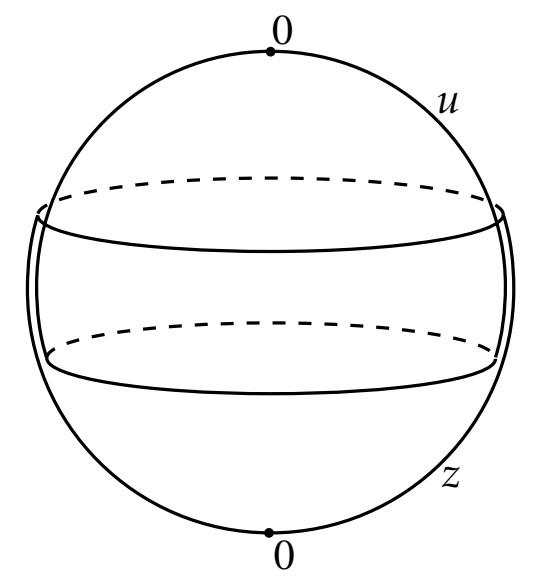
\includegraphics[width=0.5\textwidth]{figure/Fig6.1.jpg}\\
		\caption{A sphere constructed from the $z$ and $u$ coordinate charts .}\label{fig:6.1}
	\end{center}
\end{figure}

The sphere $S_2$ can be covered by two coordinate charts, as shown in figure \ref{fig:6.1} . We take disks $|z|<\rho$ and $|u|<\rho$, where $\rho>1$, and glue them via :
\begin{equation}
	u=1 / z  \label{6.1.1}
\end{equation}
\begin{tcolorbox}[breakable]
	\begin{proof}
		Consider \( x \in \mathbb{R}^n \), and define stereographic projection from the \textbf{north pole} of the unit sphere \( S^n \subset \mathbb{R}^{n+1} \) as:
		
		\[
		X^i = \frac{2x^i}{1 + |x|^2}, \quad
		X^{n+1} = \frac{|x|^2 - 1}{1 + |x|^2}
		\]
		where $x^i$ are coordinates on the plane and $X^i$ are the coordiantes on the sphere in embedding space. Now project this point on the sphere back to \( \mathbb{R}^n \) via stereographic projection from the \textbf{south pole}:
		
		\[
		x'^i = \frac{X^i}{1 + X^{n+1}}
		\]
		Substituting:
		
		\[
		x'^i = \frac{\frac{2x^i}{1 + |x|^2}}{1 + \frac{|x|^2 - 1}{1 + |x|^2}}
		= \frac{2x^i}{(1 + |x|^2) + (|x|^2 - 1)} = \frac{2x^i}{2|x|^2} = \frac{x^i}{|x|^2}
		\]
		Hence, the composition $(\mathbb{R}^n \xrightarrow{\text{north}} \mathbb{S}^n \xrightarrow{\text{south}} \mathbb{R}^n)$ gives:
		
		\[
		x^i \mapsto \frac{x^i}{|x|^2}
		\]
		which is the \textbf{inversion} in the unit sphere.
	\end{proof}
\end{tcolorbox}
In fact, we can take $\rho \to \infty$ . In this way, the coordinate $z$ is well-defined everywhere except at the "North Pole" $u=0$ . We can view the sphere as a Riemann surface by taking flat metrics on both coordinate charts and connecting them with a conformal (coordinate plus Weyl) transformation . Alternatively, we can view it as a Riemannian manifold with a globally defined metric . The general conformal gauge metric is :
\begin{equation}
	\dif s^{2}=\exp (2 \omega(z, \bar{z})) \dif z \dif \bar{z} \:. \label{6.1.2}
\end{equation}
Since $\dif z \dif \bar{z}=|z|^{4} \dif u \dif \bar{u}$, the condition for this metric to be non-singular at $u=0$ is that $\exp (2 \omega(z, \bar{z}))$ decays as $|z|^{-4}$ as $z \to \infty$ . For example :
\begin{equation}
	\dif s^{2}=\frac{4 r^{2}\, \dif z \dif \bar{z}}{(1+z \bar{z})^{2}}=\frac{4 r^{2}\, \dif u \dif \bar{u}}{(1+u \bar{u})^{2}} \label{6.1.3}
\end{equation}
describes a sphere with radius $r$ and curvature $R=2 / r^{2}$ .

According to the general discussion in section \ref{sec:5.2}, the sphere has no moduli but has 6 CKVs, making every metric ($\text{diff} \times \text{Weyl}$) equivalent to \eqref{6.1.3} . We observe this at the infinitesimal level . As in \eqref{5.2.8}, we look for holomorphic tensor fields $\delta g_{z z}(z)$ and holomorphic vector fields $\delta z(z)$ . These must be defined on the entire sphere, so we examine the transformation to the $u$ coordinate chart :
\begin{subequations}  \label{6.1.4}
	\begin{align}
		\delta u &=\frac{\partial u}{\partial z} \delta z=-z^{-2} \delta z \:, \label{6.1.4a} \\
		\delta g_{u u} &=\left(\frac{\partial u}{\partial z}\right)^{-2} \delta g_{z z}=z^{4} \delta g_{z z} \:. \label{6.1.4b} 
	\end{align}
\end{subequations}
Any holomorphic quadratic differential $\delta g_{z z}$ must be holomorphic with respect to $z$ and vanish as $z^{-4}$ at infinity; therefore, it must be identically zero . On the other hand, the CKV $\delta z$ being holomorphic at $u=0$ requires it to grow no faster than $z^{2}$ as $z \rightarrow \infty$ . Thus, the general CKV is :
\begin{subequations} \label{6.1.5}
	\begin{align}
		\delta z       &= a_{0}+a_{1} z+a_{2} z^{2}  \:, \label{6.1.5a} \\
		\delta \bar{z} &= a_{0}^{*}+a_{1}^{*} \bar{z}+a_{2}^{*} \bar{z}^{2} \:, \label{6.1.5b}
	\end{align}
\end{subequations}
which has 3 complex parameters or 6 real parameters, exactly as expected from the Riemann-Roch theorem . Exponentiating these infinitesimal transformations gives the \emph{Möbius group} :
\begin{equation}
	z^{\prime}=\frac{\alpha z+\beta}{\gamma z+\delta} \:. \label{6.1.6}
\end{equation}
Rescaling $\alpha, \beta, \gamma, \delta$ does not change the transformation, so we can fix $\alpha \delta-\beta \gamma=1$ and treat the set under global sign inversion of $\alpha, \beta, \gamma, \delta$ as equivalent, which defines the $PSL(2, \mathds{C})$ group . This is the most general coordinate transformation that is holomorphic on the entire $S_2$  . it is a one-to-one mapping including the point at infinity . Three of the six parameters correspond to ordinary rotations, forming the subgroup $SO(3)$ of $PSL(2, \mathds{C})$ .

\subsection*{The Disk}

The disk $D_2$ can be constructed from the sphere by identifying two points under reflection . For example, identify $z$ and $z^{\prime}$ such that :
\begin{equation}
	z^{\prime}=1 / \bar{z} \:. \label{6.1.7}
\end{equation}
In polar coordinates $z=r \me^{\mi \phi}$, this takes the reciprocal of the radius but preserves the angle, so the unit disk $|z| \leq 1$ is the fundamental domain after gluing . Points on the unit circle are fixed by the reflection, so it becomes a boundary . It is often more convenient to use the conformally equivalent inversion :
\begin{equation}
	z^{\prime}=\bar{z}  \label{6.1.8}
\end{equation}
Now the upper half-plane is the fundamental domain, and the real axis is the boundary .

The CKG of the disk is the subgroup of $PSL(2, \mathds{C})$ that keeps the boundary of the disk invariant . For the inversion \eqref{6.1.8}, this is the subgroup where $\alpha, \beta, \gamma, \delta$ in \eqref{6.1.6} are all real, namely $PSL(2, \mathds{R})$, the Möbius group of real parameters . One CKV is the ordinary rotational symmetry on the disk . Once again, all metrics are equivalent, and there are no moduli .

\subsection*{The Projective Plane}

The projective plane $RP_2$ can also be obtained as a $\mathds{Z}_{2}$ identification of the sphere . Glue points $z$ and $z^{\prime}$ such that :
\begin{equation}
	z^{\prime}=-1 / \bar{z} \label{6.1.9}
\end{equation}
These points are antipodal points in the round metric \eqref{6.1.3} . There are no fixed points, so there is no boundary in the resulting space, but the space is non-orientable . A fundamental domain for this gluing is the unit disk $|z| \leq 1$, but points $\me^{\mi \phi}$ and $-\me^{\mi \phi}$ are identified . Another choice is the upper $z$-plane, where there are no moduli . The CKG is the subgroup of $PSL(2, \mathds{C})$ reflecting the \eqref{6.1.9} identification; this is the ordinary rotation group $SO(3)$ . Both the disk and the projective plane can be represented as spheres with points identified under a $\mathds{Z}_{2}$ transformation or \emph{involution} . In fact, every worldsheet can be obtained from a closed oriented surface by identification under one or two $\mathds{Z}_{2}$ involutions . Thus, Green's functions can be obtained using the method of images .

\section{Expectation values of scalars} \label{sec:6.2}

The basic quantities we need are the expectation values of vertex operators . To develop several useful techniques and viewpoints, we will calculate them in three different ways: direct path integrals, using holomorphy, and the operator method later in this chapter .

The path integral method has already been used for the Faddeev-Popov determinant in section \ref{sec:5.3} and for the harmonic oscillator in the appendix . Starting from a general functional :
\begin{equation}
	Z[J]=\left\langle\exp \left(\mi \int \dif^{2} \sigma\: J(\sigma) \cdot X(\sigma)\right)\right\rangle \label{6.2.1}
\end{equation}
where $J_{\mu}(\sigma)$ is arbitrary . From now on, we work on an arbitrary compact two-dimensional surface $M$, and the spacetime dimension is $d$ . We expand $X^{\mu}(\sigma)$ on a complete basis $\mathsf{X}_{I}(\sigma)$ :
\begin{subequations} \label{6.2.2}
	\begin{align}
		X^{\mu}(\sigma) &= \sum_{I} x_{I}^{\mu} \mathsf{X}_{I}(\sigma) \:, \label{6.2.2a} \\
		\nabla^{2} \mathsf{X}_{I} &= -\omega_{I}^{2} \mathsf{X}_{I} \:,  \label{6.2.2b} \\
		\int_{M} \dif^{2} \sigma\: g^{1 / 2} \mathsf{X}_{I} \mathsf{X}_{I^{\prime}} &= \delta_{I I^{\prime}} \:. \label{6.2.2c} 
	\end{align}	
\end{subequations}
Then :
\begin{equation}
	Z[J]=\prod_{I, \mu} \int \dif x_{I}^{\mu} \exp \left(-\frac{\omega_{I}^{2} x_{I}^{\mu} x_{I \mu}}{4 \pi \alpha^{\prime}}+\mi x_{I}^{\mu} J_{I \mu}\right) \:, \label{6.2.3}
\end{equation}
where :
\begin{equation}
	J_{I}^{\mu}=\int \dif^{2} \sigma J^{\mu}(\sigma) \mathsf{X}_{I}(\sigma) \:. \label{6.2.4}
\end{equation}
Except for the constant mode :
\begin{equation}
	\mathsf{X}_{0}=\left(\int \dif^{2} \sigma \: g^{1 / 2}\right)^{-1 / 2} \:, \label{6.2.5}
\end{equation}
this integral is Gaussian . The action for the constant mode is zero, so it yields a $\delta$-function .

\begin{tcolorbox}
	\begin{remark}
		For $I=0$, \eqref{6.2.3} gives :
		\[
		\int \dif x^{\mu}_{0} \: \exp (\mi x^{\mu}_{0}J_{0\mu}) \propto \delta^{d}(J_{0}) \:.
		\]
	\end{remark}
\end{tcolorbox}
\noindent Evaluating the integral yields :
\begin{align}
	Z[J] &= \mi(2 \pi)^{d} \delta^{d}(J_{0}) \prod_{I \neq 0} \left(\frac{4 \pi^{2} \alpha^{\prime}}{\omega_{I}^{2}}\right)^{d / 2} \exp \left(-\frac{\pi \alpha^{\prime} J_{I} \cdot J_{I}}{\omega_{I}^{2}}\right) \nonumber  \\
	&= \mi(2 \pi)^{d} \delta^{d}\left(J_{0}\right)\left(\operatorname{det}^{\prime} \frac{-\nabla^{2}}{4 \pi^{2} \alpha^{\prime}}\right)^{-d / 2} \nonumber  \\
	& \qquad \quad \times \exp \left(-\frac{1}{2} \int \dif^{2} \sigma \, \dif^{2} \sigma^{\prime}\: J(\sigma) \cdot J(\sigma^{\prime}) 
	G^{\prime}(\sigma, \sigma^{\prime})\right) \:. \label{6.2.6}
\end{align}
As discussed in sections \ref{sec:2.1} and \ref{sec:3.2}, the Gaussian integral generated by the timelike mode $x_{I}^{0}$ has the wrong sign, so it is defined via contour rotation $x_{I}^{0} \to-\mi x_{I}^{d}, I \neq 0$ . The primed Green's function removes the zero-mode contribution :
\begin{equation}
	G^{\prime}(\sigma_{1}, \sigma_{2})=\sum_{I \neq 0} \frac{2 \pi \alpha^{\prime}}{\omega_{I}^{2}} \mathsf{X}_{I}(\sigma_{1}) \mathsf{X}_{I}(\sigma_{2}) \:. \label{6.2.7}
\end{equation}
It satisfies the differential equation :
\begin{align}
	-\frac{1}{2 \pi \alpha^{\prime}} \nabla^{2} G^{\prime}(\sigma_{1}, \sigma_{2}) 
	&=\sum_{I \neq 0} \mathsf{X}_{I}(\sigma_{1}) \mathsf{X}_{I}(\sigma_{2})  \nonumber \\
	&=g^{-1 / 2} \delta^{2}(\sigma_{1}-\sigma_{2})-\mathsf{X}_{0}^{2}  \:, \label{6.2.8}
\end{align}
where the completeness of $\mathsf{X}_{I}$ is used . An ordinary Green's function with a $\delta$-function source does not exist . It would correspond to the electrostatic potential of a single charge, but on a compact surface, field lines flowing out of the source have nowhere to go . The $\mathsf{X}_{0}^{2}$ term can be viewed as a background charge distribution used to neutralize the system .

\subsection*{The Sphere}
Specifically on the sphere, the solution to the differential equation \eqref{6.2.8} is :
\begin{equation}
	G^{\prime}(\sigma_{1}, \sigma_{2})=-\frac{\alpha^{\prime}}{2} \ln |z_{12}|^{2}+f(z_{1}, \bar{z}_{1})+f(z_{2}, \bar{z}_{2}) \:. \label{6.2.9}
\end{equation}
\begin{tcolorbox}
	\begin{remark}
		On the sphere $g=\me^{4 \omega}$, $\nabla^{2}=\me^{-2 \omega} \partial \bar{\partial}$, so \eqref{6.2.8} becomes :
		\[
		\partial \bar{\partial} G^{\prime}=-2 \pi \alpha^{\prime} \delta^{2}(\sigma_{1}-\sigma_{2})
		+2 \pi \alpha^{\prime} \me^{2 \omega}\,\mathsf{X}_{0}^{2} 
		\]
		where $\partial \bar{\partial} \ln |z_{12}|^{2}=2 \pi \delta^{2}(z, \bar{z})=4 \pi \delta^{2}(\sigma_{1}-\sigma_{2})$ .
	\end{remark}
\end{tcolorbox}
\noindent where :
\begin{equation}
	f(z, \bar{z})=\frac{\alpha^{\prime} \mathsf{X}_{0}^{2}}{4} 
	\int \dif^{2} z^{\prime}\: \exp [2 \omega(z^{\prime}, \bar{z}^{\prime})] \ln|z-z^{\prime}|^{2}+k \:. \label{6.2.10}
\end{equation}
The condition that $G^{\prime}$ is orthogonal to $\mathsf{X}_{0}$ determines the constant $k$, but in any case, we will see that all expectation values is independent of the function $f$. It originates from the background charge, but the $\delta$-function from the zero-mode integration forces overall neutrality, $J_{0}^{\mu}=0$, so the background field has no net contribution .

Now consider the path integral containing a product of tachyon vertex operators :
\begin{equation}
	A_{S_{2}}^{n}(k, \sigma)=\left\langle\left[\me^{\mi k_{1} \cdot X(\sigma_{1})}\right]_{\mathrm{r}}
	\left[\me^{\mi k_{2} \cdot X(\sigma_{2})}\right]_{\mathrm{r}} \cdots
	\left[\me^{\mi k_{n} \cdot X(\sigma_{n})}\right]_{\mathrm{r}}\right\rangle_{S_{2}} \:. \label{6.2.11}
\end{equation}
This corresponds to :
\begin{equation}
	J(\sigma)=\sum_{i=1}^{n} k_{i} \delta^{2}(\sigma-\sigma_{i}) \:. \label{6.2.12}
\end{equation}
Then the amplitude \eqref{6.2.6} becomes :
\begin{align}
	A_{S_{2}}^{n}(k, \sigma) &=\mi C_{S_{2}}^{X}(2 \pi)^{d} \delta^{d}({\textstyle \sum_{i}} k_{i}) \nonumber \\
	& \quad \times \exp \Biggl(-\sum_{ i<j}^{n} k_{i} \cdot k_{j} G^{\prime}(\sigma_{i}, \sigma_{j})
	-\frac{1}{2} \sum_{i=1}^{n} k_{i}^{2} G_{\mathrm{r}}^{\prime}(\sigma_{i}, \sigma_{i})\Biggr) \:. \label{6.2.13}
\end{align}
The constant here is :
\begin{equation}
	C_{S_{2}}^{X}=\mathsf{X}_{0}^{-d}\left(\operatorname{det}^{\prime} \frac{-\nabla^{2}}{4 \pi^{2} \alpha^{\prime}}\right)_{S_{2}}^{-d/2} 
	\:. \label{6.2.14}
\end{equation}
\begin{tcolorbox}
	\begin{remark}
		According to \eqref{6.2.4} and \eqref{6.2.5}, $J_{0}=\int \dif^{2} \sigma \: \mathsf{X}_{0} J(\sigma)= \mathsf{X}_{0} \sum_{i} k_{i}$, so $\delta^{d}(J_{0})=\mathsf{X}_{0}^{-d} \delta^{d}(\sum_{i} k_{i})$ .
	\end{remark}
\end{tcolorbox}
\noindent The determinant can be regularized and calculated, but we do not need to calculate it explicitly . We adopt the renormalization from section \ref{sec:3.6} such that self-contractions include :
\begin{equation}
	G_{\mathrm{r}}^{\prime}(\sigma, \sigma^{\prime})=G^{\prime}(\sigma, \sigma^{\prime})
	+\frac{\alpha^{\prime}}{2} \ln d^{2}(\sigma, \sigma^{\prime}) \:. \label{6.2.15}
\end{equation}
Note that :
\begin{equation}
	G_{\mathrm{r}}^{\prime}(\sigma, \sigma)=2 f(z, \bar{z})+\alpha^{\prime} \omega(z, \bar{z}) \label{6.2.16}
\end{equation}
is finite . Then the path integral on the sphere is :
\begin{equation}
	A_{S_{2}}^{n}(k, \sigma)=\mi C_{S_{2}}^{X}(2 \pi)^{d} \delta^{d}({\textstyle \sum_{i}} k_{i}) 
	\exp \left(-\frac{\alpha^{\prime}}{2} \sum_{i} k_{i}^{2} \omega\left(\sigma_{i}\right)\right) 
	\prod_{i<j}|z_{i j}|^{\alpha^{\prime} k_{i} \cdot k_{j}} \:. \label{6.2.17}
\end{equation}
The dependence on the conformal factor $\omega(\sigma)$ is obtained from the Weyl anomaly of the vertex operators . For on-shell operators, it will cancel the variation of $g^{1/2}$ . We will take the metric to be flat (pushing the curvature to infinity) in a large region containing all vertex operators; thus, terms in $\omega(\sigma_{i})$ are dropped .
\begin{tcolorbox}[breakable]
	Notes on \eqref{6.2.16}:
	\[
	\ln d^{2}(\sigma, \sigma^{\prime})-\ln |z_{12}|^{2}=
	\ln \left(\frac{\int \me^{2 \omega} \: \dif z \dif \bar{z}}{\int \dif z \dif  \bar{z}}\right)=2 \omega	
	\]
	Notes on \eqref{6.2.17}: Taking $n=2$ as an example, the part depending on $f$ is 
	\[
	k_{1} k_{2} (f_{1}+f_{2})+\frac{1}{2} k_{1}^{2} \cdot 2 f_{1}+\frac{1}{2} k_{2}^{2} \cdot 2 f_{2} 
	=(k_{1} f_{1}+k_{2} f_{2})(k_{1}+k_{2})
	\]
	Since the path integral contains $\delta(\sum_{i} k_{i})= k_{1}+k_{2}$, it is independent of $f$ .
\end{tcolorbox}

Higher-order vertex operators are exponentials multiplied by partial derivatives of $X^{\mu}$, so we further need :
\begin{equation}
	\Biggl\langle\prod_{i=1}^{n}\left[\me^{\mi k_{i} \cdot X(z_{i}, \bar{z}_{i})}\right]_{\mathrm{r}} 
	\prod_{j=1}^{p} \partial X^{\mu_{j}}(z_{j}^{\prime}) \prod_{k=1}^{q} \bar{\partial} X^{\nu_{k}}(\bar{z}_{k}^{\prime \prime})\Biggr\rangle \biggr._{\!\!S_{2}} \:. \label{6.2.18}
\end{equation}
This is given by summing over all contractions, where each $\partial X$ or $\bar{\partial} X$ must contract with an exponential or other $\partial X$ and $\bar{\partial} X$ . The $XX$ contraction is $-\frac{1}{2} \alpha^{\prime} \ln |z|^{2}$, and $f$ is again dropped in the final expression . This result is summarized as :
\begin{align}
	&\mi C_{S_{2}}^{X}(2 \pi)  \delta^{d}({\textstyle\sum_{i} }k_{i}) 
	\exp\Biggl(-\frac{\alpha'}{2}\sum_{i}k_{i}^{2}\omega(\sigma_{i})\Biggr)
	\prod_{i<j}^{n}|z_{i j}|^{\alpha^{\prime} k_{i} \cdot k_{j}}  \nonumber \\
	& \qquad \quad \times\Biggl\langle 
	\prod_{j=1}^{p}\Bigl[v^{\mu_{j}}(z_{j}^{\prime})+q^{\mu_{j}}(z_{j}^{\prime})\Bigr] 
	\prod_{k=1}^{q}\Bigl[\tilde{v}^{\nu_{k}}(\bar{z}_{k}^{\prime \prime})+\tilde{q}^{\nu_{k}}(\bar{z}_{k}^{\prime \prime})\Bigr]\Biggr\rangle  \label{6.2.19}
\end{align}
where :
\begin{equation}
	v^{\mu}(z)=- \mi \frac{\alpha^{\prime}}{2} \sum_{i=1}^{n} \frac{k_{i}^{\mu}}{z-z_{i}}, \qquad 
	\tilde{v}^{\mu}(\bar{z})=-\mi \frac{\alpha^{\prime}}{2} \sum_{i=1}^{n} \frac{k_{i}^{\mu}}{\bar{z}-\bar{z}_{i}} \label{6.2.20}
\end{equation}
originate from contractions with the exponentials . The expectation value of $q^{\mu}=\partial X^{\mu}-v^{\mu}$ is given by contraction with $-\eta^{\mu \nu}(z-z^{\prime})^{-2} \alpha^{\prime} / 2$ and summing, while the expectation value of $\tilde{q}^{\nu}$ is given by conjugation .
\begin{tcolorbox}[breakable]
	\begin{proof}
The operator product can be expanded as following:
\begin{align}
	\prod_{i=1}^{n}\normal{&\bigl[\me^{\mi k_i\cdot X(z_i,\bar z_i)}\bigr]_{\mathrm r}}
	\prod_{j=1}^{p}\normal{\partial X^{\mu_j}(z'_j)}
	\prod_{k=1}^{q}\normal{\bar\partial X^{\nu_k}(\bar z''_k)}
	\nonumber\\[4pt]
	&=\sum_{i=1}^{n}
	\contraction{}{\partial X^{\mu_1}(z'_1)}{\,}{e^{\mi k_i\cdot X(z_i,\bar z_i)}}
	\partial X^{\mu_1}(z'_1)e^{\mi k_i\cdot X(z_i,\bar z_i)}
	\normal{
		\prod_{\substack{l=1\\ l\neq i}}^{n}\bigl[\me^{\mi k_l\cdot X(z_l,\bar z_l)}\bigr]_{\mathrm r}
		\prod_{j=2}^{p}\partial X^{\mu_j}(z'_j)
		\prod_{k=1}^{q}\bar\partial X^{\nu_k}(\bar z''_k)}
	\nonumber\\
	&\qquad+\sum_{j=2}^{p}
	\wick{\partial \c1 X^{\mu_1}(z'_1)\partial \c1 X^{\mu_j}(z'_j)}
	\normal{
		\prod_{i=1}^{n}\bigl[\me^{\mi k_i\cdot X(z_i,\bar z_i)}\bigr]_{\mathrm r}
		\prod_{\substack{l=2\\ l\neq j}}^{p}\partial X^{\mu_l}(z'_l)
		\prod_{k=1}^{q}\bar\partial X^{\nu_k}(\bar z''_k)}
	\nonumber\\
	&\qquad+\sum_{k=1}^{q}
	\wick{\partial \c1 X^{\mu_1}(z'_1)\bar\partial \c1 X^{\nu_k}(\bar z''_k)}
	\normal{
		\prod_{i=1}^{n}\bigl[\me^{\mi k_i\cdot X(z_i,\bar z_i)}\bigr]_{\mathrm r}
		\prod_{j=2}^{p}\partial X^{\mu_j}(z'_j)
		\prod_{\substack{l=1\\ l\neq k}}^{q}\bar\partial X^{\nu_l}(\bar z''_l)}
	\nonumber\\[6pt]
	&\qquad+\sum_{i=1}^{n}
	\contraction{}{\bar\partial X^{\nu_1}(\bar z''_1)}{\,}{e^{\mi k_i\cdot X(z_i,\bar z_i)}}
	\bar\partial X^{\nu_1}(\bar z''_1)e^{\mi k_i\cdot X(z_i,\bar z_i)}
	\normal{
		\prod_{\substack{l=1\\ l\neq i}}^{n}\bigl[\me^{\mi k_l\cdot X(z_l,\bar z_l)}\bigr]_{\mathrm r}
		\prod_{j=1}^{p}\partial X^{\mu_j}(z'_j)
		\prod_{k=2}^{q}\bar\partial X^{\nu_k}(\bar z''_k)}
	\nonumber\\
	&\qquad+\sum_{k=2}^{q}
	\wick{\bar\partial \c1 X^{\nu_1}(\bar z''_1)\bar\partial \c1 X^{\nu_k}(\bar z''_k)}
	\normal{
		\prod_{i=1}^{n}\bigl[\me^{\mi k_i\cdot X(z_i,\bar z_i)}\bigr]_{\mathrm r}
		\prod_{j=1}^{p}\partial X^{\mu_j}(z'_j)
		\prod_{\substack{l=2\\ l\neq k}}^{q}\bar\partial X^{\nu_l}(\bar z''_l)}
	\nonumber\\
	&\qquad+\sum_{j=1}^{p}
	\wick{\bar\partial \c1 X^{\nu_1}(\bar z''_1)\partial \c1 X^{\mu_j}(z'_j)}
	\normal{
		\prod_{i=1}^{n}\bigl[\me^{\mi k_i\cdot X(z_i,\bar z_i)}\bigr]_{\mathrm r}
		\prod_{\substack{l=1\\ l\neq j}}^{p}\partial X^{\mu_l}(z'_l)
		\prod_{k=2}^{q}\bar\partial X^{\nu_k}(\bar z''_k)}.
\end{align}
Each holomorphic $\del X^\mu(z')$ (or anti holomorphic term $\bar\del X^\mu(z')$) upon contraction with the vertex operator generates the classical function $v^\mu$ times the vertex operator itself:
		\begin{align}
			\sum_{i=1}^n \contraction{}{X^\mu(z')}{\,}{e^{i k_i \cdot X(z_i)}}
			 \partial X^\mu(z') e^{i k_i \cdot X(z_i)}		
			&= \sum_{i=1}^n \left( i k_i^\rho \expval{\del X^\mu(z') X_\rho(z_i)} \right) \normal{\prod e^{ik \cdot X}} \nonumber \\
			&= \underbrace{\sum_{i=1}^n \left( - \frac{i \alpha'}{2} \frac{k_i^\mu}{z' - z_i} \right)}_{v^\mu(z')} \normal{\prod e^{ik \cdot X}}
		\end{align}
		Since the vertex operator are left over one can further contract it with the remaining operators in the same term. Each contraction appears as a factor of $v^{\mu}$ or $\bar v^{\mu}$. Contraction of vertex operator in those terms produce $\normal{\ldots}$ which annihilate the vacuum due to absence of commuting zero mode and hence drop out. To evaluate the contraction between $\partial X$, we need
		\begin{equation}
			\wick{ \c1 {\del X^\mu(z_1')} \c1 {\del X^\nu(z_2')} } 
			= \expval{q^\mu(z_1') q^\nu(z_2')} 
			= -\frac{\alpha'}{2} \frac{\eta^{\mu\nu}}{(z_1' - z_2')^2}
		\end{equation}
		and the last expression to evaluate the contraction between vertex operator is:
		\begin{equation}
			\wick{ \c1 {\normal{e^{i k_i \cdot X(z_i)}}} \c1 {\normal{e^{i k_j \cdot X(z_j)}}} } 
			= \exp\left( -k_i \cdot k_j \expval{X(z_i) X(z_j)} \right)
			= |z_i - z_j|^{\alpha' k_i \cdot k_j}
		\end{equation}
		To implement this efficiently, we will follow the following decomposition to isolate the contraction with $e^{ik\cdot  X}$ to write the result cleanly. 
		\begin{equation}
			\del X^\mu(z') \to v^\mu(z') + q^\mu(z')
		\end{equation}
		where $v^\mu(z')$ originates from contraction with $e^{ik\cdot  X}$ and $q^\mu(z')$ only contracts with other $q^\mu(z')$. Combining all factors, including the normalization $C_{S_2}^X$ and the regularization term $\omega(z)$, the amplitude is:
		
		\begin{align}
			A_{S_{2}} &= \mathcal{C}_{S_{2}}^{X}(2 \pi)  \delta^{d}\left(\sum k_{i}\right) 
			\exp\left(-\frac{\alpha'}{2}\sum_{i}k_{i}^{2}\omega(z_{i})\right)
			\prod_{i<j}^{n}|z_{i j}|^{\alpha^{\prime} k_{i} \cdot k_{j}} \nonumber \\
			&\quad \times \expval{ 
				\prod_{j=1}^{p} \left[ v^{\mu_{j}}(z_{j}^{\prime}) + q^{\mu_{j}}(z_{j}^{\prime}) \right] 
				\prod_{k=1}^{q} \left[ \tilde{v}^{\nu_{k}}(\bar{z}_{k}^{\prime \prime}) + \tilde{q}^{\nu_{k}}(\bar{z}_{k}^{\prime \prime}) \right] 
			}
		\end{align}
		QED.
	\end{proof}
\end{tcolorbox}
Now we re-calculate in a different way, using holomorphy . As an example, consider :
\begin{equation}
	\langle\partial X^{\mu}(z_{1}) \partial X^{\nu}(z_{2})\rangle_{S_{2}} \:. \label{6.2.21}
\end{equation}
The OPE determines it to be :
\begin{equation}
	-\frac{\alpha^{\prime} \eta^{\mu \nu}}{2 z_{12}^{2}}\langle 1\rangle_{S_{2}}+g(z_{1}, z_{2}) \:, \label{6.2.22}
\end{equation}
where $g(z_{1}, z_{2})$ is holomorphic in both variables . In the $u$ coordinate chart :
\begin{equation}
	\partial_{u} X^{\mu}=-z^{2} \partial_{z} X^{\mu} \:, \label{6.2.23}
\end{equation}
so the condition for holomorphy at $u=0$ is that the expectation value of $\partial_{z} X^{\mu}$ decays as $z^{-2}$ as $z$ goes to infinity . More generally, the behavior of a tensor with weight $(h, 0)$ at infinity is $z^{-2 h}$ . Focusing on the correlation of \eqref{6.2.22} with respect to $z_{1}$ at fixed $z_{2}$, this implies $g(z_{1}, z_{2})$ decays as $z_{1}^{-2}$ at infinity, hence the holomorphic factor is zero . Compared with the path integral result \eqref{6.2.19}, this is consistent . Although $\langle 1\rangle_{S_{2}}$ seems to diverge like $\delta(0)$, this is just the zero-mode divergence from the infinite spacetime volume . Regarding the expectation value of a product of vertex operators :
\begin{equation}
	A_{S_{2}}^{n}(k, \sigma)=\left\langle\prod_{i=1}^{n}:\mathrel{\me^{\mi k_{i} \cdot X(z_{i}, \bar{z}_{i})}}:\right\rangle \Big._{\!S_{2}}
	\label{6.2.24}
\end{equation}
calculating with this method is less direct because they are not holomorphic . In fact, they factorize into holomorphic and anti-holomorphic parts, but this is subtle and is best introduced in the language of operators, which we will do in chapter \ref{cha:8} . We use the holomorphy of the translation current . Consider the expectation value with an additional current $\partial X^{\mu}(z)$ . The OPE of the current and vertex operators determines the singularity at $z$ :
\begin{equation}
	\left\langle\partial X^{\mu}(z) \prod_{i=1}^{n}:\mathrel{\me^{\mi k_{i} \cdot X(z_{i}, \bar{z}_{i})}}:\right
	\rangle\bigg._{\!S_{2}}=-\frac{\mi \alpha^{\prime}}{2} A_{S_{2}}^{n}(k, \sigma) \sum_{i=1}^{n} \frac{k_{i}^{\mu}}{z-z_{i}} 
	+\text{terms holomorphic at } z \:. \label{6.2.25}
\end{equation}
\begin{tcolorbox}
	\begin{proof}
		Use
		\begin{equation}
		\sum_{i=1}^{n}\contraction{}{X^\mu(z')}{\,}{e^{i k_i \cdot X(z_i)}}\partial X^\mu(z') e^{i k_i \cdot X(z_i)}	= \left( - \frac{i \alpha'}{2} \frac{k_i^\mu}{z' - z_i} \right) \normal{\prod_{i=1}^{n} e^{ik \cdot X}}
		\end{equation}
	\end{proof}
\end{tcolorbox}
Now observe $z \rightarrow \infty$ . The condition that $\partial_{u} X^{\mu}$ is holomorphic at $u=0$ again requires this expectation value to vanish as $z^{-2}$ as $z \rightarrow \infty$ . Then the holomorphic terms in \eqref{6.2.25} are zero, and the term at order $z^{-1}$ is zero . We find momentum conservation :
\begin{equation}
	A_{S_{2}}^{n}(k, \sigma) \sum_{i=1}^{n} k_{i}^{\mu}=0 \:. \label{6.2.26}
\end{equation}
We state this in a slightly different way . Consider the contour integral of the spacetime translation current :
\begin{equation}
	p^{\mu}=\frac{1}{2 \pi \mi} \oint_{C}(\dif z \: j_{z}^{\mu}-\dif \bar{z}\: j_{\bar{z}}^{\mu}) \:, \label{6.2.27}
\end{equation}
where the contour $C$ encloses all exponential operators . There are two ways to calculate it . One is to shrink the contour $C$ until it becomes a small circle around each vertex operator, which picks out the $(z-z_{i})^{-1}$ term from each OPE and gives $\sum_{i=1}^{n} k_{i}^{\mu}$ . The other is to expand it until it is a small circle on the $u$ coordinate chart: due to holomorphy at $u=0$, it must be zero . This discussion of deforming contours is widely used in CFT . We have used the OPE to determine singularities and then used holomorphy to completely determine the dependence on $z$ . Now let us look at the second term of the OPE as $z \rightarrow z_{1}$ . Expanding \eqref{6.2.25} gives :
\begin{equation}
	-\frac{\mi \alpha^{\prime}}{2} A_{S_{2}}^{n}(k, \sigma)\left(\frac{k_{1}^{\mu}}{z-z_{1}}+\sum_{i=2}^{n} \frac{k_{i}^{\mu}}{z_{1}-z_{i}}+O(z-z_{1})\right) \:. \label{6.2.28}
\end{equation}
\begin{tcolorbox}[breakable]
	\begin{proof}
		Use 
		\begin{align}
			\frac{1}{z-z_i} &=\frac{1}{z_1-z_i}\frac{z_1-z_i}{z-z_i}=\frac{1}{z_1-z_i}\frac{1}{1+\frac{z-z_1}{z_1-z_i}}=\frac{1}{z_1-z_i}+O(z-z_1)
		\end{align}
		in \eqref{6.2.25}
	\end{proof}
\end{tcolorbox}
Contracting with $\mi k_{1}^{\mu}$, the $(z-z_{1})^{0}$ order term must be consistent with the OPE :
\begin{align}
	\mi k_{1} \cdot \partial X(z): \mathrel{\me^{\mi k_{1} \cdot X(z_{1}, \bar{z}_{1})}}: =\frac{\alpha^{\prime} k_{1}^{2}}{2(z-z_{1})} :\mathrel{\me^{\mi k_{1} \cdot X(z_{1}, \bar{z}_{1})}}:
	+ \: \partial_{z_{1}}{:\mathrel{\me^{\mi k_{1} \cdot X(z_{1}, \bar{z}_{1})}}:}+ O(z-z_{1}) \:. \label{6.2.29}
\end{align}
This implies :
\begin{equation}
	\partial_{z_{1}} A_{S_{2}}^{n}(k, \sigma)=\frac{\alpha^{\prime}}{2} A_{S_{2}}^{n}(k, \sigma) \sum_{i=2}^{n} \frac{k_{1} \cdot k_{i}}{z_{1 i}} \:. \label{6.2.30}
\end{equation}
Integrating and using conjugate equations as well as momentum conservation . In the sense of normalization difference, this determines the path integral :
\begin{equation}
	A_{S_{2}}^{n}(k, \sigma) \propto \delta^{d}({\textstyle \sum_{i} k_{i}}) 
	\prod_{i<j}^{n} |z_{i j}|^{\alpha^{\prime} k_{i} \cdot k_{j}} \:, \label{6.2.31}
\end{equation}
which is consistent with the first method . Note that for comparison, we must push the curvature to infinity ($\omega(\sigma_{i})=0$), which makes $[]_{\mathrm{r}}=::$ .
\begin{tcolorbox}
	\begin{remark}
		Note that \eqref{6.2.31} does satisfy \eqref{6.2.30} with
		\begin{equation}
			\partial_z [z_{1i}^{\frac{\alpha' k_1\cdot k_i}{2}}] = \frac{\alpha'k_1\cdot k_i}{2} \frac{z_{1i}}{z_1-z_i}
		\end{equation}
	\end{remark}
\end{tcolorbox}
It is worth noting that the intermediate steps of the path method depend on the specific choice of the Riemann metric . This metric is needed to preserve coordinate invariance in these steps . Two different metrics, if Weyl equivalent, still give different Laplacians and eigenfunctions . But in the end, in string theory, these correlations must be dropped . The second method uses only the fundamental properties of the Riemann surface, its holomorphy .

\subsection*{The Disk}
The extension to the disk is direct . By taking the representation of the sphere above and constraining $z$ to the upper complex plane, we obtain the representation of the disk . The Neumann boundary term is interpreted as an image charge :
\begin{equation}
	G^{\prime}(\sigma_{1}, \sigma_{2})=-\frac{\alpha^{\prime}}{2} \ln |z_{1}-z_{2}|^{2}
	-\frac{\alpha^{\prime}}{2} \ln |z_{1}-\bar{z}_{2}|^{2} \:, \label{6.2.32}
\end{equation}
differing by a term that is dropped due to momentum conservation . Then :
\begin{align}
	\left\langle\prod_{i=1}^{n}: \mathrel{\me^{\mi k_{i} \cdot X(z_{i}, \bar{z}_{i})}}:\right\rangle \bigg._{\!\!D_{2}} 
	=& \mi C_{D_{2}}^{X} (2 \pi)^{d} \delta^{d}({\textstyle\sum_{i} k_{i}}) 
	\prod_{i=1}^{n}|z_{i}-\bar{z}_{i}|^{\alpha^{\prime} k_{i}^{2} / 2}  \nonumber \\
	& \times \prod_{ i<j}^{n} |z_{i}-z_{j}|^{\alpha^{\prime} k_{i} \cdot k_{j} }
	|z_{i}-\bar{z}_{j}|^{\alpha^{\prime} k_{i} \cdot k_{j}} \:. \label{6.2.33}
\end{align}
For expectation values containing $\partial_{a} X^{\mu}$, one again sums over contractions, but now using the Green's function \eqref{6.2.32} . Note that $\partial X^{\mu}(z) \bar{\partial} X^{\nu}(\bar{z}^{\prime})$ (or $q^{\mu}(z) \tilde{q}^{\nu}(\bar{z}^{\prime})$) has a non-zero contraction .

For two points on the boundary, the two terms in the Green's function \eqref{6.2.32} are equal; even after subtracting the first term in normal ordering, the Green's function still diverges at zero interval . For this reason, boundary operators must be defined using boundary normal ordering, where the subtraction is doubled :
\begin{equation}
	\bno X^{\mu}(y_{1}) X^{\nu}(y_{2})\bno = X^{\mu}(y_{1}) X^{\nu}(y_{2})+2 \alpha^{\prime} \eta^{\mu \nu} 
	\ln |y_{1}-y_{2}| \:,  \label{6.2.34}
\end{equation}
where $y$ represents coordinates on the real axis . Combinatorics is the same as for other forms of normal ordering . The expectation values of boundary normal ordered boundary operators have the same well-behaved properties (no singularities) as internal conformal normal ordered operators .
\begin{tcolorbox}[breakable]
	\begin{remark}
A more intuitive way to see why the standard normal ordering fails on the disk boundary is to use the \textbf{method of images}. On the disk \(D_2\), the Green's function for a free boson with Neumann (or Dirichlet) boundary conditions can be written as a sum of a direct term and an image term:

\begin{equation}
	\langle X(z_1) X(z_2) \rangle \sim -\frac{\alpha'}{2} \ln |z_1 - z_2|^2 \;-\; \frac{\alpha'}{2} \ln |z_1 - \bar{z}_2|^2 + \text{finite}.\label{prop}
\end{equation}

The first term is the usual bulk propagator; the second term comes from the image charge at \(\bar{z}_2\) needed to satisfy the boundary condition (e.g., Neumann on the real axis). 

On the boundary, we have \(z = \bar{z}\). Therefore, when both points are on the boundary, \(z_1\) and \(z_2\) are real, and
\begin{equation}
	|z_1 - \bar{z}_2|^2 = |z_1 - z_2|^2.
\end{equation}

Thus the propagator \eqref{prop} restricted to the boundary becomes
\begin{equation}
	\langle X(z_1) X(z_2) \rangle \big|_{\partial} \sim -\alpha' \ln |z_1 - z_2|^2 + \text{finite}.
\end{equation}

The standard normal ordering subtracts only \(\frac{\alpha'}{2} \ln |z_1 - z_2|^2\), which is \emph{half} of the actual singularity. Consequently, the normal‑ordered product retains a residual divergence:

\begin{equation}
	\langle :X(z_1)X(z_2): \rangle \big|_{\partial} \sim -\frac{\alpha'}{2} \ln |z_1 - z_2|^2 + \text{finite}.
\end{equation}

The boundary normal ordering \(\bno \cdots \bno\) is defined to subtract the \emph{full} boundary singularity:

\begin{equation}
	\bno X(y_1) X(y_2) \bno = X(y_1) X(y_2) + 2\alpha' \ln(y_1 - y_2).
\end{equation}
which renders the correlators finite on the boundary.
\end{remark}
\end{tcolorbox}
If an expectation value contains both boundary exponentials and internal exponentials, each with appropriate normal ordering, drop the $|z_{i}-\bar{z}_{i}|^{\alpha^{\prime} k_{i}^{2} / 2}$ factor for the boundary operators and take the appropriate limit of the internal result \eqref{6.2.33} . Explicitly, for exponentials all on the boundary :
\begin{equation}
	\left\langle\prod_{i=1}^{n} \bno \me^{\mi k_{i} \cdot X(y_{i})} \bno \right\rangle\bigg._{\!\!D_{2}}
	=\mi C_{D_{2}}^{X}(2 \pi)^{d} \delta^{d}(\textstyle{\sum_{i} k_{i}} ) 
	\prod_{i<j}^{n}|y_{i}-y_{j}|^{2 \alpha^{\prime} k_{i} \cdot k_{j}} \:. \label{6.2.35}
\end{equation}
More generally :
\begin{align}
	& \left\langle\prod_{i=1}^{n} \bno \me^{\mi k_{i} \cdot X(y_{i})} \bno 
	\prod_{j=1}^{p} \partial_{y}X^{\mu_{j}}(y_{j}^{\prime})\right\rangle\bigg._{\!\!D_{2}}
	= \mi C_{D_{2}}^{X}(2 \pi)^{d} \delta^{d}({\textstyle \sum_{i} k_{i}})  \nonumber \\
	&\qquad \qquad \qquad \qquad  \times \prod_{i<j}^{n}|y_{i j}|^{2 \alpha^{\prime} k_{i} \cdot k_{j}}
	\left\langle\prod_{j=1}^{p}\Bigl[v^{\mu_{j}}(y_{j}^{\prime})+q^{\mu_{j}}(y_{j}^{\prime})\Bigr]\right\rangle\bigg._{\!\!D_{2}} \:, 
	\label{6.2.36}
\end{align}
where :
\begin{equation}
	v^{\mu}(y)=-2 \mi \alpha^{\prime} \sum_{i=1}^{n} \frac{k_{i}^{\mu}}{y-y_{i}} \label{6.2.37}
\end{equation}
and $q$ is contracted with $-2 \alpha^{\prime}(y-y^{\prime})^{-2} \eta^{\mu \nu}$ .

\subsection*{The Projective Plane}
The Green's function given by the method of images is :
\begin{equation}
	G^{\prime}(\sigma_{1}, \sigma_{2})=-\frac{\alpha^{\prime}}{2} \ln |z_{1}-z_{2}|^{2}
	-\frac{\alpha^{\prime}}{2} \ln |1+z_{1} \bar{z}_{2}|^{2} \:. \label{6.2.38}
\end{equation}
Now :
\begin{align}
	\left\langle\prod_{i=1}^{n}:\mathrel{\me^{\mi k_{i} X(z_{i}, \bar{z}_{i})}}:\right\rangle\bigg._{\!\! RP_{2}} 
	&=\mi C_{RP_{2}}^{X}(2 \pi)^{d} \delta^{d}({\textstyle\sum_{i} k_{i}}) 
	\prod_{i=1}^{n}|1+z_{i} \bar{z}_{i}|^{\alpha^{\prime} k_{i}^{2} / 2} \nonumber \\
	&\quad  \times \prod_{i<j}^{n}|z_{i}-z_{j}|^{\alpha^{\prime} k_{i} \cdot k_{j}}|1+z_{i} \bar{z}_{j}|^{\alpha^{\prime} k_{i} k_{j}} \:, \label{6.2.39}
\end{align}
and similarly for more general expectation values . Since there are no fixed points, it is impossible for point $z$ to touch its image $-\bar{z}^{-1}$, so there is no boundary .
\begin{tcolorbox}[breakable]
	\begin{proof}
		Starting from the Sphere Green's function in \eqref{6.2.9}, we  add an image term identifying $z_2\to-\frac{1}{\bar z_2}$
		\begin{equation}
			G^{\prime}(\sigma_{1}, \sigma_{2})=-\frac{\alpha^{\prime}}{2} \ln |z_{1}-z_{2}|^{2} \:
		\end{equation}
		This gives us \eqref{6.2.39}. Then using \eqref{6.2.13}, we write
		\begin{equation}
			\left\langle \prod_{i=1}^n :e^{i k_i\cdot X(z_i,\bar z_i)}: \right\rangle_{RP_2}
			=
			\exp\!\left(
			-\sum_{i<j} k_i\cdot k_j\, G'(\sigma_i,\sigma_j)
			-\frac12 \sum_i k_i^2\, G'_{\rm reg}(\sigma_i,\sigma_i)
			\right)\left\langle e^{i\sum_i k_i\cdot x_0}\right\rangle
		\end{equation}
		where $x_0$ denotes the zero mode of $X^\mu$ and $G'_{\rm reg}(\sigma_i,\sigma_i)$ is the regularized coincident Green function. The zero-mode is given as
		\begin{equation}
			\left\langle e^{i\left(\sum_i k_i\right)\cdot x_0}\right\rangle
			=(2\pi)^d \delta^d\!\left(\sum_i k_i\right).
		\end{equation}
		The $RP_2$ Green function for $i\neq j$ is given as:
		\begin{align}
			-\;k_i\cdot k_j\,G'(\sigma_i,\sigma_j)
			&=
			\frac{\alpha'}{2}\,k_i\cdot k_j\,\ln|z_i-z_j|^2
			+\frac{\alpha'}{2}\,k_i\cdot k_j\,\ln|1+z_i\bar z_j|^2 ,
		\end{align}
		so that
		\begin{equation}
			\exp\!\left[-\sum_{i<j} k_i\cdot k_j\,G'(\sigma_i,\sigma_j)\right]
			=
			\prod_{i<j}
			|z_i-z_j|^{\alpha' k_i\cdot k_j}
			|1+z_i\bar z_j|^{\alpha' k_i\cdot k_j}.
		\end{equation}
		
		For the coincident limit, normal ordering removes the singular term
		$-\frac{\alpha'}{2}\ln|z_i-z_i|^2$, but the image term survives. Hence
		\begin{equation}
			G'_{\rm reg}(\sigma_i,\sigma_i)
			=
			-\frac{\alpha'}{2}\ln|1+z_i\bar z_i|^2,
		\end{equation}
		and therefore
		\begin{align}
			\exp\!\left[-\frac12 \sum_i k_i^2\,G'_{\rm reg}(\sigma_i,\sigma_i)\right]
			&=
			\prod_i
			\exp\!\left(\frac{\alpha'}{4}k_i^2\ln|1+z_i\bar z_i|^2\right) \\
			&=
			\prod_i |1+z_i\bar z_i|^{\alpha' k_i^2/2}.
		\end{align}
		
		Combining all factors, we obtain
		\begin{align}
			\left\langle\prod_{i=1}^{n}:\!e^{i k_{i}\cdot X(z_{i}, \bar z_{i})}\!:\right\rangle_{RP_{2}}
			&=
			i\,C_{RP_{2}}^{X}(2 \pi)^{d} \delta^{d}\!\left(\sum_{i} k_{i}\right)
			\prod_{i=1}^{n}|1+z_{i} \bar{z}_{i}|^{\alpha^{\prime} k_{i}^{2} / 2} \nonumber \\
			&\quad \times
			\prod_{i<j}^{n}
			|z_{i}-z_{j}|^{\alpha^{\prime} k_{i}\cdot k_{j}}
			|1+z_{i}\bar{z}_{j}|^{\alpha^{\prime} k_{i}\cdot k_{j}} .
		\end{align}
	\end{proof}
\end{tcolorbox}
\section{$bc$ Conformal Field Theory} \label{sec:6.3}

\subsection*{The Sphere}

The path integral for ghost fields has already been established in section \ref{sec:5.3} . According to the Riemann-Roch theorem, the simplest non-zero expectation value is :
\begin{equation}
	\langle c(z_{1}) c(z_{2}) c(z_{3}) \tilde{c}(\bar{z}_{4}) \tilde{c}(\bar{z}_{5}) \tilde{c}(\bar{z}_{6})\rangle_{S_{2}} \:. \label{6.3.1}
\end{equation}
Up to normalization (i.e., a functional determinant), the result \eqref{5.3.18} is the zero-mode determinant :
\begin{equation}
	\operatorname{det} \mathsf{C}_{0 j}^{a}(\sigma_{i}) \:. \label{6.3.2}
\end{equation}
Six CKVs were found in section \ref{sec:6.1} . In the complex basis, they are :
\begin{subequations} \label{6.3.3}
	\begin{align}
		\mathsf{C}^{z} &= 1, z, z^{2}\:, \quad \mathsf{C}^{\bar{z}}=0  \:, \label{6.3.3a} \\
		\mathsf{C}^{z} &= 0\:, \quad \mathsf{C}^{\bar{z}}=1, \bar{z}, \bar{z}^{2} \:. \label{6.3.3b}
	\end{align}
\end{subequations}
In this basis, the determinant splits into two $3 \times 3$ blocks, and the expectation value becomes :
\begin{equation}
	C_{S_{2}}^{\mathrm{g}} \operatorname{det}\left|\begin{array}{ccc}
		1 & 1 & 1 \\
		z_{1} & z_{2} & z_{3} \\
		z_{1}^{2} & z_{2}^{2} & z_{3}^{2}
	\end{array}\right| \operatorname{det}\left|\begin{array}{ccc}
		1 & 1 & 1 \\
		\bar{z}_{4} & \bar{z}_{5} & \bar{z}_{6} \\
		\bar{z}_{4}^{2} & \bar{z}_{5}^{2} & \bar{z}_{6}^{2}
	\end{array}\right|=C_{S_{2}}^{\mathrm{g}} z_{12} z_{13} z_{23} \bar{z}_{45} \bar{z}_{46} \bar{z}_{56} \:. \label{6.3.4}
\end{equation}
The constant $C_{S_{2}}^{\mathrm{g}}$ contains the functional determinant and the finite-dimensional Jacobian (independent of position); the Jacobian arises because the basis \eqref{6.3.3} is not orthogonal .

For tree-level amplitudes, this is the only $bc$ path integral we need, but for completeness, we give :
\begin{align}
	\left\langle\prod_{i=1}^{p+3} c(z_{i}) \prod_{j=1}^{p} b(z_{j}^{\prime}) \cdot(\text{anti-holomorphic})\right\rangle\bigg._{\!\!S_{2}}
	&=C_{S_{2}}^{\mathrm{g}} \frac{z_{p+1, p+2} z_{p+1, p+3} z_{p+2, p+3}}{(z_{1}-z_{1}^{\prime}) \cdots(z_{p}-z_{p}^{\prime})} \cdot(\text {anti-holomorphic})  \nonumber \\
	&\qquad \qquad \pm \text {permutations} \:, \label{6.3.5}
\end{align}
which is completed by contracting $b$ and $c$ . The anti-holomorphic part has the same form . We do not care about the overall sign; for the Faddeev-Popov determinant in any case, we will take the absolute value .

To provide another derivation using holomorphy, once again, let us first examine the conservation law . The conservation law can be obtained by inserting the ghost number contour integral $\oint_{C} \dif z \: j(z) / 2 \pi \mi$ into the amplitude \eqref{6.3.5}, where $C$ encloses all vertex operators and the ghost number current is $j=-:\mathrel{bc}:$ . From the OPE of $b$ and $c$, this merely counts the number of $c$ fields minus the number of $b$ fields, giving $n_{c}-n_{b}$ times the original amplitude . Now use the conformal transformation \eqref{2.5.17} to pull the contour back to the $u$ coordinate chart :
\begin{equation}
	\oint_{C} \frac{\dif z}{2 \pi \mi}\, j_{z}=-\oint_{C} \frac{\dif u}{2 \pi \mi}\, j_{u}+3 \to 3 \:. \label{6.3.6}
\end{equation}
The offset $+3$ is because $j$ is not a tensor, and its OPE with $T$ contains a $z^{-3}$ term . In the last step, we used holomorphy in the $u$ coordinate chart . The non-zero amplitude thus has $n_{c}-n_{b}=3$ and similarly $n_{\tilde{c}}-n_{\tilde{b}}=3$, which is consistent with the Riemann-Roch theorem .

From the OPE, the ghost expectation value \eqref{6.3.1} is holomorphic with respect to each value, and it must be zero when two identical anticommuting fields come together . Therefore, it must be of the form :
\begin{equation}
	z_{12} z_{13} z_{23} \bar{z}_{45} \bar{z}_{46} \bar{z}_{56} F(z_{1}, z_{2}, z_{3}) 
	\tilde{F}(\bar{z}_{4}, \bar{z}_{5}, \bar{z}_{6}) \:, \label{6.3.7}
\end{equation}
where $F$ and $\tilde{F}$ are holomorphic and anti-holomorphic functions of position, respectively . As $z_{1} \rightarrow \infty$, it tends to $z_{1}^{2} F$ . However, $c$ is a tensor with weight $-1$, so the amplitude cannot be greater than $z_{1}^{2}$ at infinity . Thus $F(z_{i})$ must be independent of $z_{1}$, and similarly for $z_{2}$ and $z_{3}$ . The discussion for $\tilde{F}$ is similar, and we again obtain the result \eqref{6.3.4} . For the general case \eqref{6.3.5}, the same discussion gives the result :
\begin{equation}
	C_{S_{2}}^{\mathrm{g}} \prod_{i<i^{\prime}}^{p+3} z_{i i^{\prime}} \prod_{j<j^{\prime}}^{p} z_{j j^{\prime}}^{\prime} 
	\prod_{i=1}^{p+3} \prod_{j=1}^{p}(z_{i}-z_{j}^{\prime})^{-1} \cdot(\text {anti-holomorphic}) \:, \label{6.3.8}
\end{equation}
which has the correct poles, zeros, and correct behavior at infinity . Summing the permutations in \eqref{6.3.5} obviously gives this term . We considered only $\lambda=2$, which is related to the ghosts of the bosonic string, but both methods can be readily generalized to any $\lambda$ .

\subsection*{The Disk}
The simplest way to obtain the $bc$ amplitude on the disk is the doubling trick . As in \eqref{2.7.30}, we can represent the holomorphic and anti-holomorphic fields on the upper half-plane using holomorphic fields on the entire plane . Using :
\begin{equation}
	\tilde{b}(\bar{z})=b(z^{\prime}), \quad \tilde{c}(\bar{z})=c(z^{\prime}), \quad z^{\prime}=\bar{z},\:\: \operatorname{Im} z>0 \:. \label{6.3.9}
\end{equation}
The expectation value of holomorphic fields is obtained as for the sphere :
\begin{equation}
	\langle c(z_{1}) c(z_{2}) c(z_{3})\rangle_{D_{2}}=C_{D_{2}}^{\mathrm{g}} z_{12} z_{13} z_{23} \:. \label{6.3.10}
\end{equation}
For example :
\begin{align}
	\langle c(z_{1}) c(z_{2}) \tilde{c}(\bar{z}_{3})\rangle_{D_{2}} 
	&=\langle c(z_{1}) c(z_{2}) c(z_{3}^{\prime})\rangle_{D_{2}} \nonumber \\
	&=C_{D_{2}}^{\mathrm{g}} z_{12}(z_{1}-\bar{z}_{3})(z_{2}-\bar{z}_{3}) \:. \label{6.3.11}
\end{align}
More general correlation functions are obtained in the same way .

\subsection*{The Projective Plane}

The doubling trick can be used again . The inversion $z^{\prime}=-\bar{z}^{-1}$ implies :
\begin{equation}
	\tilde{b}(\bar{z})=\left(\frac{\partial z^{\prime}}{\partial \bar{z}}\right)^{2} b(z^{\prime})=z^{\prime 4} b(z^{\prime})\:, \quad 
	\tilde{c}(\bar{z})=\left(\frac{\partial z^{\prime}}{\partial \bar{z}}\right)^{-1} c(z^{\prime})=z^{\prime-2} c(z^{\prime}) \:. \label{6.3.12}
\end{equation}
Once again :
\begin{equation}
	\langle c(z_{1}) c(z_{2}) c(z_{3})\rangle_{RP_{2}}=C_{R P_{2}}^{\mathrm{g}} z_{12} z_{13} z_{23} \label{6.3.13}
\end{equation}
and :
\begin{align}
	\langle c(z_{1}) c(z_{2}) \tilde{c}(\bar{z}_{3})\rangle_{R P_{2}} 
	&=z_{3}^{\prime-2} \langle c(z_{1}) c(z_{2}) c(z_{3}^{\prime})\rangle_{R P_{2}} \nonumber \\
	&=C_{R P_{2}}^{\mathrm{g}} z_{12}(1+z_{1} \bar{z}_{3})(1+z_{2} \bar{z}_{3}) \:. \label{6.3.14}
\end{align}
\begin{tcolorbox}
	\begin{remark}
		The last step of the above equation :
		\begin{align*}
			z_{3}^{\prime-2} \cdot C_{R P_{2}}^{g}(z_{1}-z_{2})(z_{1}-z_{3}^{\prime})(z_{2}-z_{3}^{\prime}) 
			&= \bar{z}_{3}^{2} C_{R P_{2}}^{g}(z_{1}-z_{2})(z_{1}+\bar{z}_{3}^{-1})(z_{2}+\bar{z}_{3}^{-1}) \\
			&= C_{R P_{2}}^{g}(z_{1}-z_{2})(1+z_{1} \bar{z}_{3})(1+z_{2} \bar{z}_{3}) \:.
		\end{align*}
	\end{remark}
\end{tcolorbox}



\section{The Veneziano amplitude} \label{sec:6.4}

Open string amplitudes are simpler than closed string amplitudes, so we begin with them .

We represent the disk as the upper half-plane, so the boundary coordinate $y$ is real . There are no moduli . After fixing the metric, the CKG $PSL(2, \mathds{R})$ can be used to fix three vertex operators to arbitrary positions $y_{1}, y_{2}, y_{3}$ on the boundary, except that the group does not change the cyclic order of the vertex operators, so we sum over two orders . For three open string tachyons on the disk, the general expression for the string $S$-matrix \eqref{5.3.9} reduces to :
\begin{align}
	S_{D_{2}}(k_{1} ; k_{2} ; k_{3})=g_{\mathrm{o}}^{3} \me^{-\lambda}
	\Bigl\langle \bno c^1 \me^{\mi k_{1} \cdot X}(y_{1})\bno \bno c^{1} \me^{\mi k_{2} \cdot X}(y_{2})\bno 
	\bno c^{1} \me^{\mi k_{3} \cdot X}(y_{3})\bno\Bigr\rangle_{D_{2}} 
	+(k_{2} \leftrightarrow k_{3}),  \label{6.4.1}
\end{align}
where each fixed coordinate integral is replaced by the corresponding $c$ ghost . Each open string introduces a factor $g_{\mathrm{o}}$, which is the coupling constant of the open string . The factor $\me^{-\lambda}$ comes from the Euler number term in the action . Of course, $g_{\mathrm{o}}$ is related to $\me^{\lambda}$, $g_{\mathrm{o}}^{2} \propto e^{\lambda}$, but we will determine the proportionality constant as we go further . The expectation value in \eqref{6.4.1} was found in the previous section (again, taking the absolute value of the ghost fields), giving :
\begin{align}
	S_{D_{2}}(k_{1} ; k_{2} ; k_{3})&= \mi g_{\mathrm{o}}^{3} C_{D_{2}}(2 \pi)^{26} \delta^{26}({\textstyle \sum_{i} k_{i}}) \nonumber  \\
	&\quad \times |y_{12}|^{1+2 \alpha^{\prime} k_{1} \cdot k_{2}}|y_{13}|^{1+2 \alpha^{\prime} k_{1} \cdot k_{3}}
	|y_{23}|^{1+2 \alpha^{\prime} k_{2} \cdot k_{3}}+ (k_{2} \leftrightarrow k_{3}) \:, \label{6.4.2}
\end{align}
where $C_{D_{2}}=\me^{-\lambda} C_{D_{2}}^{X} C_{D_{2}}^{\mathrm{g}}$ . Momentum conservation and the mass-shell condition $k_{i}^{2}=1 / \alpha^{\prime}$ imply :
\begin{equation}
	2 \alpha^{\prime} k_{1} \cdot k_{2}=\alpha^{\prime}(k_{3}^{2}-k_{1}^{2}-k_{2}^{2})=-1 \label{6.4.3}
\end{equation}
The same applies to other $k_{i} \cdot k_{j}$, so this reduces to :
\begin{equation}
	S_{D_{2}}(k_{1} ; k_{2} ; k_{3})=2 \mi g_{\mathrm{o}}^{3} C_{D_{2}}(2 \pi)^{26} \delta^{26}({\textstyle\sum_{i} k_{i}}) \label{6.4.4}
\end{equation}
This is independent of the choice of gauge $y_{i}$, which is a general property of the Faddeev-Popov scheme . Weyl invariance is key—if the vertex operators were not on-shell, the amplitude would depend on the choice of $y_{i}$ .

We can also use the independence of $y_{i}$ to give the Faddeev-Popov determinant without calculation . Using the mass-shell condition and momentum conservation, the expectation value of $X^{\mu}$ is proportional to $|y_{12} y_{13} y_{23}|^{-1}$, so the measure must be its reciprocal . When the number of vertex operators $n>3$, the same measure still applies because in all these cases, three positions are fixed . The 4-tachyon amplitude is obtained in the same way :
\begin{align}
	&S_{D_{2}}(k_{1} ; k_{2} ; k_{3} ; k_{4}) \nonumber \\
	&\quad =g_{\mathrm{o}}^{4} \me^{-\lambda} \int_{-\infty}^{\infty} \dif y_{4}\:
	\left\langle\prod_{i=1}^{3} \bno c^{1}(y_{i}) \me^{\mi k_{i} \cdot X(y_{i})}\bno 
	\bno \me^{\mi k_{4} \cdot X(y_{4})}\bno \right\rangle +(k_{2} \leftrightarrow k_{3}) \nonumber \\
	&\quad =\mi g_{\mathrm{o}}^{4} C_{D_{2}}(2 \pi)^{26} \delta^{26}({\textstyle\sum_{i} k_{i}})|y_{12} y_{13} y_{23}|
	\int_{-\infty}^{\infty} \dif y_{4} \prod_{i<j}|y_{i j}|^{2 \alpha^{\prime} k_{i} \cdot k_{j}} +(k_{2} \leftrightarrow k_{3}) \:. \label{6.4.5}
\end{align}
After a variable substitution (Möbius transformation) for $y_{4}$, this is again independent of $y_{1,2,3}$ . It is customary to take $y_{1}=0, y_{2}=1$, and $y_{3} \rightarrow \infty$ . Amplitudes are usually expressed in terms of Mandelstam variables :
\begin{equation}
	s=-(k_{1}+k_{2})^{2}, \quad t=-(k_{1}+k_{3})^{2}, \quad u=-(k_{1}+k_{4})^{2} \label{6.4.6}
\end{equation}
These are not independent: momentum conservation and the mass-shell condition imply :
\begin{equation}
	s+t+u=\sum_{i} m_{i}^{2}=-\frac{4}{\alpha^{\prime}} \:. \label{6.4.7}
\end{equation}

\noindent Using $2 \alpha^{\prime} k_{i} \cdot k_{j}=-2+\alpha^{\prime}(k_{i}+k_{j})^{2}$, the amplitude becomes :
\begin{align}
	&S_{D_{2}}(k_{1} ; k_{2}; k_{3} ; k_{4}) = \mi  g_{\mathrm{o}}^{4} C_{D_{2}}(2 \pi)^{26} \delta^{26}({\textstyle\sum_{i} k_{i}})
	\nonumber \\
	&\qquad \qquad \times\left[\int_{-\infty}^{\infty} \dif y_{4}\: |y_{4}|^{-\alpha^{\prime} u-2}|1-y_{4}|^{-\alpha^{\prime} t-2}
	+(t \rightarrow s)\right] \:. \label{6.4.8}
\end{align}


\begin{figure}[!htbp]
	\begin{center}
		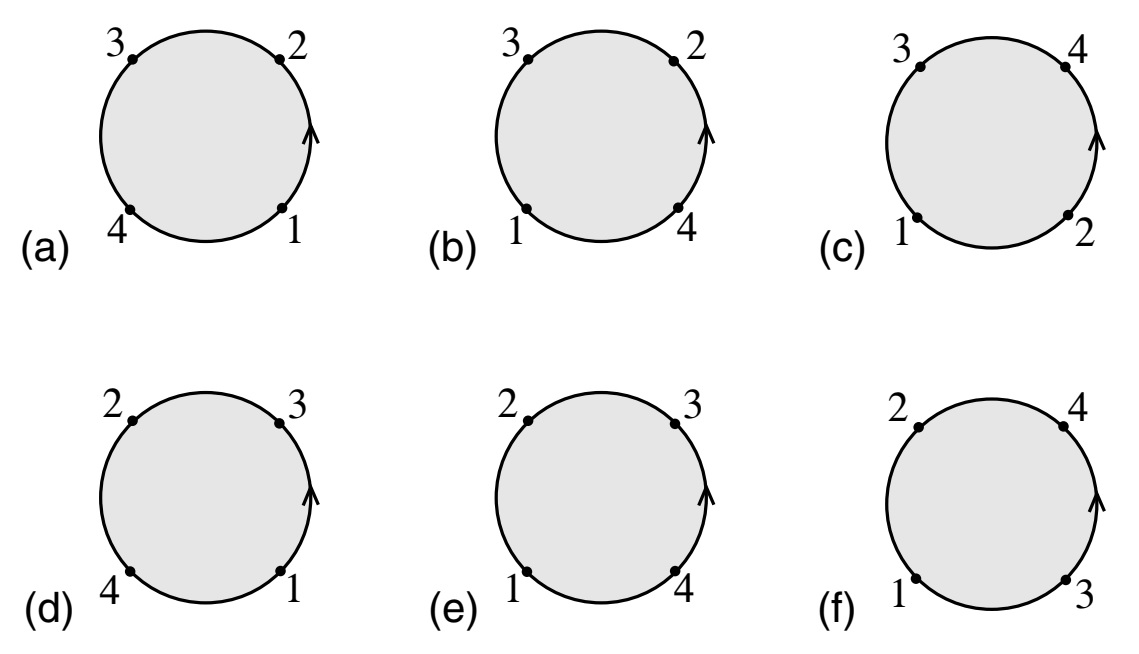
\includegraphics[width=0.5\textwidth]{figure/Fig6.2.jpg}\\
		\caption{Six cyclically inequivalent orderings of four open string vertex operators on a circle . Except for a jump from $\infty$ to $-\infty$ at point 3, the coordinate $y$ increases in the direction of the arrow .}\label{fig:6.2}
	\end{center}
\end{figure}


The integral splits into three parts, $-\infty<y_{4}<0$, $0<y_{4}<1$, and $1<y_{4}<\infty$ . For these three ranges, the ordering of vertex operators is as shown in figure \ref{fig:6.2}(a)(b)(c) . Möbius invariance can be used to transform these ranges to any other, so the contributions they give are equivalent to permutations of vertex operators . The $(t \leftrightarrow s)$ term gives figure \ref{fig:6.2}(d)(e)(f) . Taken together :
\begin{equation}
	S_{D_{2}}(k_{1} ; k_{2} ; k_{3} ; k_{4}=2 \mi g_{\mathrm{o}}^{4} C_{D_{2}}(2 \pi)^{26} \delta^{26}({\textstyle\sum_{i} k_{i}})
	[I(s, t)+I(t, u)+I(u, s)] \:, \label{6.4.9}
\end{equation}
where :
\begin{equation}
	I(s, t)=\int_{0}^{1} \dif y\: y^{-\alpha^{\prime} s-2}(1-y)^{-\alpha^{\prime} t-2}  \:. \label{6.4.10}
\end{equation}
These three terms come from figures \ref{fig:6.2} (c)(f), (b)(d), and (a)(e), respectively .

If $\alpha^{\prime} s<-1$ and $\alpha^{\prime} t<-1$, the integral $I(s,t)$ converges . As $\alpha^{\prime} s \rightarrow-1$, the integral diverges at $y=0$ . To study this divergence, take a neighborhood of $y=0$ and approximate the integrand :
\begin{align}
	I(s, t) &=\int_{0}^{r} d y y^{-\alpha^{\prime} s-2}+\text{terms analytic at } \alpha^{\prime} s=-1   \nonumber \\
	&=-\frac{r^{-\alpha^{\prime} s-1}}{\alpha^{\prime} s+1}+\text{terms analytic at } \alpha^{\prime} s=-1 \nonumber\\
	&=-\frac{1}{\alpha^{\prime} s+1}+\text{terms analytic at } \alpha^{\prime} s=-1 \:. \label{6.4.11}
\end{align}
In \eqref{6.4.11}, we calculated the integral in the convergence region . We see that this divergence is a pole at $s=-1 / \alpha^{\prime}$, the mass square of the open string tachyon . The variable $s$ is exactly the center-of-mass energy squared for the scattering $1+2 \rightarrow 3+4$, so this pole is a resonance produced by intermediate tachyon states . Once again, this is an artifact of the bosonic string, i.e., the lightest string state is a tachyon, which is irrelevant to the discussion . This pole is due to the process in figure \ref{fig:6.3}(a) . There, tachyons 1 and 2 merge into a single tachyon, then split back into tachyons 3 and 4 .

\begin{figure}[!htbp]
	\begin{center}
		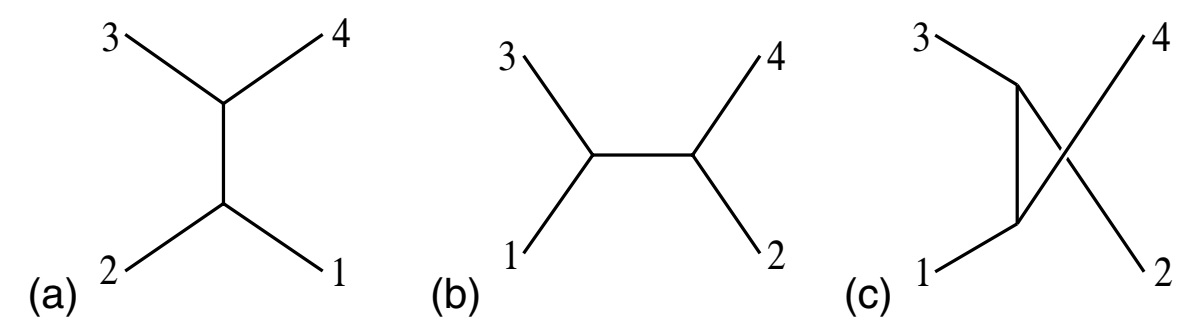
\includegraphics[width=0.5\textwidth]{figure/Fig6.3.jpg}\\
		\caption{Processes giving poles in the (a) $s$-, (b) $t$-, and (c) $u$-channels .}\label{fig:6.3}
	\end{center}
\end{figure}

Since the singularity at $\alpha^{\prime} s=-1$ is only a pole, $I(s,t)$ can be analytically continued around this point and into the region $\alpha^{\prime} s>-1$ . The amplitude is defined via analytic continuation . The divergence of the amplitude at this pole is a significant physical feature: the resonance corresponding to an intermediate string state propagating over long spacetime distances . Divergence bypassing this pole is not; it is merely an artifact of this specific integral representation of the amplitude . Continuation poses no problem . In fact, we will see that every string divergence is of this basic form, so this analytic continuation removes all divergences—except, of course, the divergence of the pole itself . The pole is on the real axis, and we need to define it more precisely . For Minkowski processes, the correct $\epsilon$ treatment is :
\begin{equation}
	\frac{1}{\alpha^{\prime} s+1}  \equiv \frac{1}{\alpha^{\prime} s+1+i \epsilon} 
	\equiv \mathrm{P} \frac{1}{\alpha^{\prime} s+1}- \mi \pi \delta (\alpha^{\prime} s+1) \:, \label{6.4.12}
\end{equation}
where $\mathrm{P}$ represents the principal value . Unitarity (which we will systematically develop in chapter \ref{cha:9}) requires this pole to appear, and determines the coefficient from the scattering amplitude of two tachyons to one string :
\begin{equation}
	S_{D_{2}}(k_{1} ; k_{2} ; k_{3} ; k_{4})= \mi \int \frac{\dif^{26} k}{(2 \pi)^{26}} 
	\frac{S_{D_{2}}(k_{1} ; k_{2} ; k) S_{D_{2}}(-k ; k_{3} ; k_{4})}{-k^{2}+\alpha^{\prime-1}+ \mi \epsilon} 
	+\text{ terms analytic at } k^{2}=\frac{1}{\alpha^{\prime}}\:. \label{6.4.13}
\end{equation}

Gathering factors in the 4-tachyon amplitude, including the equivalent contribution of $I(u, s)$ to this pole, and using the 3-tachyon result \eqref{6.4.4}, condition \eqref{6.4.13} gives :
\begin{equation}
	C_{D_{2}}=\me^{-\lambda} C_{D_{2}}^{X} C_{D_{2}}^{\mathrm{g}}=\frac{1}{\alpha^{\prime} g_{\mathrm{o}}^{2}} \:. \label{6.4.14}
\end{equation}
\begin{tcolorbox}
	\begin{remark}
		Singular term given by \eqref{6.4.13} :
		\[
		\mi \cdot(2 \mi g_{\mathrm{o}}^{3} C_{D_{2}})^{2}(2 \pi)^{26} \alpha^{\prime} 
		\delta^{2 b}({\textstyle\sum_{i} k_{i}}) \frac{1}{\alpha^{\prime} s+1} \:,
		\]
		Singular term given by \eqref{6.4.9} :
		\[
		2 \cdot 2 \mi g_{\mathrm{o}}^{4} C_{D_{2}}(2 \pi)^{26} \delta^{26}({\textstyle\sum_{i} k_{i}}) \frac{-1}{\alpha^{\prime} s+1}\:.
		\]
		The two together give \eqref{6.4.14} .
	\end{remark}
\end{tcolorbox}
\noindent Then the 3-tachyon amplitude is :
\begin{equation}
	S_{D_{2}}(k_{1} ; k_{2} ; k_{3})=\frac{2 \mi g_{\mathrm{o}}}{\alpha^{\prime}}(2 \pi)^{26} \delta^{26}({\textstyle\sum_{i} k_{i}}) \:. 
	\label{6.4.15}
\end{equation}
Various functional determinants are dropped . Using unitarity, all normalizations can be expressed in terms of the coupling $g_o$ appearing in vertex operators . In fact, the determinants can also be calculated through careful regularization and renormalization, and the relative normalization of different topologies is consistent with results derived from unitarity .

Continuing analytically around the pole, we encounter further singularities . Expanding the integrand at $y=0$ :
\begin{equation}
	I(s, t)=\int_{0}^{r} \dif y\: \Bigl[y^{-\alpha^{\prime} s-2}+ (\alpha^{\prime} t+2) y^{-\alpha^{\prime} s-1}+\cdots\Bigr] \:. \label{6.4.16}
\end{equation}
The second term gives the pole at $\alpha^{\prime} s=0$ :
\begin{equation}
	I(s, t)=\frac{u-t}{2 s}+\text{terms analytic at } \alpha^{\prime} s=0 \:. \label{6.4.17}
\end{equation}
From subsequent terms in the Taylor expansion, poles of the amplitude are at :
\begin{equation}
	\alpha^{\prime} s=-1,0,1,2, \ldots \:. \label{6.4.18}
\end{equation}
These are exactly the positions of open string states . The integral $I(s, t)$ has poles in variable $t$ at the same positions \eqref{6.4.18}, which come from endpoint $y=1$ . This is due to the process in figure \ref{fig:6.3}(b) . Other two terms in the amplitude \eqref{6.4.9} give poles in the $s$-, $t$-, and $u$-channels (figure \ref{fig:6.3}c) . Because the residue of \eqref{6.4.17} at $s=0$ is odd with respect to $u-t$, this pole will actually cancel with the pole in $I(s, u)$ . Singularities at even multiples of $1 / \alpha^{\prime}$ all exhibit this behavior . But for the more general open string theory introduced in the next section, this no longer holds . Defining the Euler beta function :
\begin{equation}
	B(a, b)=\int_{0}^{1} \dif y\: y^{a-1}(1-y)^{b-1} \:, \label{6.4.19}
\end{equation}
makes :
\begin{equation}
	I(s, t)=B(-\alpha_{\mathrm{o}}(s),-\alpha_{\mathrm{o}}(t)), \qquad \alpha_{\mathrm{o}}(x)=1+\alpha^{\prime} x \:. 
	\label{6.4.20}
\end{equation}
This can be expressed as gamma functions . For fixed $w$, define $y=v / w$, which gives :
\begin{equation}
	w^{a+b-1} B(a, b)=\int_{0}^{w} \dif v \: v^{a-1}(w-v)^{b-1} \:. \label{6.4.21}
\end{equation}
Multiplying both sides by $\me^{-w}$ and integrating $\int_{0}^{\infty} \dif w$, reassembling gives :
\begin{align}
	\Gamma(a+b) B(a, b) &=\int_{0}^{\infty} \dif v\: v^{a-1} \me^{-v} \int_{0}^{\infty} \dif(w-v) \: (w-v)^{b-1} \me^{-(w-v)} \nonumber \\
	&=\Gamma(a) \Gamma(b) \:. \label{6.4.22}
\end{align}
Then the 4-tachyon amplitude is :
\begin{align}
	&S_{D_{2}}(k_{1}; k_{2} ; k_{3} ; k_{4})=\frac{2 \mi g_{\mathrm{o}}^{2}}{\alpha^{\prime}}
	(2 \pi)^{26} \delta^{26}({\textstyle \sum_{i} k_{i}}) \nonumber \\
	&\qquad \times\Bigl[B(-\alpha_{\mathrm{o}}(s),-\alpha_{\mathrm{o}}(t))+B(-\alpha_{\mathrm{o}}(s),-\alpha_{\mathrm{o}}(u))
	+B(-\alpha_{\mathrm{o}}(t),-\alpha_{\mathrm{o}}(u))\Bigr] \:, \label{6.4.23}
\end{align}
where :
\begin{equation}
	B(-\alpha_{\mathrm{o}}(x),-\alpha_{\mathrm{o}}(y))=
	\frac{\Gamma(-\alpha^{\prime} x-1) \Gamma(-\alpha^{\prime} y-1)}{\Gamma(-\alpha^{\prime} x-\alpha^{\prime} y-2)} \:. \label{6.4.24}
\end{equation}
This is the Veneziano amplitude, originally written down to model certain features of strong interactions .

The high-energy behavior of the Veneziano amplitude is important . There are two interesting regions: the Regge limit ,
\begin{equation}
	s \rightarrow \infty, \quad t \text{ fixed} \:, \label{6.4.25}
\end{equation}
and the hard scattering limit :
\begin{equation}
	s \rightarrow \infty, \quad t / s \text{ fixed} \:. \label{6.4.26}
\end{equation}
If we consider the scattering process $1+2 \rightarrow 3+4$ (so that $k_{1}^{0}$ and $k_{2}^{0}$ are positive, and $k_{3}^{0}$ and $k_{4}^{0}$ are negative)  , then in the center-of-mass frame of $1$-$2$ :
\begin{equation}
	s=E^{2}, \quad t=(4 m^{2}-E^{2}) \sin^{2}\frac{\theta}{2}, \quad u=(4 m^{2}-E^{2}) \cos ^{2} \frac{\theta}{2} \:, \label{6.4.27}
\end{equation}
where $E$ is the center-of-mass frame energy, and $\theta$ is the angle between particles 1 and 3 . The Regge limit is high energy at a small angle, while the hard scattering limit is high energy at a fixed angle . Using Stirling's approximation, $\Gamma(x+1) \approx x^{x} \me^{-x}(2 \pi x)^{1 / 2}$, behavior in the Regge region is :
\begin{equation}
	S_{D_{2}}(k_{1} ; k_{2} ; k_{3} ; k_{4}) \propto s^{\alpha_{\mathrm{o}}(t)} \Gamma(-\alpha_{0}(t)) \:, \label{6.4.28}
\end{equation}
where $\alpha_{\mathrm{o}}(t)=\alpha^{\prime} t+1$, i.e., the amplitude varies as a power of $s$, where the power depends on $t$ . This is Regge behavior . At the poles of the gamma function, the amplitude is an integer power of $s$, corresponding to exchanging a string with integer spin $\alpha_o(t)$ .

In the hard scattering limit :
\begin{equation}
	S_{D_{2}}(k_{1} ; k_{2} ; k_{3} ; k_{4}) \approx \exp \bigl[-\alpha^{\prime}(s \ln s \alpha^{\prime}+t \ln t \alpha^{\prime}+u \ln u \alpha^{\prime})\bigr]=\exp [-\alpha^{\prime} s f(\theta)] \:, \label{6.4.29}
\end{equation}
where :
\begin{equation}
	f(\theta) \approx-\sin ^{2} \frac{\theta}{2} \ln \sin ^{2} \frac{\theta}{2}-\cos ^{2} \frac{\theta}{2} \ln \cos ^{2} \frac{\theta}{2}
	\label{6.4.30}
\end{equation}
is positive . \eqref{6.4.29} is noteworthy . High-energy, fixed-angle scattering probes the internal structure of the scattered objects . Rutherford discovered the atomic nucleus using hard $\alpha$ atom scattering . Hard electron-nucleon scattering at SLAC revealed the quark components of nucleons . In quantum field theory, hard scattering amplitudes decay according to a power law in $s$ . Even for a composite object like a nucleon, if its components are point-like, its amplitude follows a power law . The exponential decay \eqref{6.4.29} is much softer, reflecting an object with a size of $\alpha^{1 / 2}$, which is what we expect .

We started from 3-point amplitudes, skipping zero-, one-, and two-point amplitudes . We will discuss these amplitudes and their interpretations in section \ref{sec:6.6} .

\section{Chan-Paton factors and gauge interactions} \label{sec:6.5}

In this section, we will examine the interactions of massless vector states of the open string . To make this discussion more interesting, we first generalize the open string theory .

At the end of chapter \ref{cha:3}, we introduced a broad class of bosonic string theories, but in our preliminary examination of interactions, we focused on the simple case of 26-dimensional flat spacetime . We can think about it in terms of symmetry: this theory has a massive 26-dimensional Poincaré invariance . In the closed bosonic string, this is the only theory with this symmetry . The proof is summarized as follows: worldsheet Noether currents of spacetime translations have components with weights (1,0) and (0,1) . By the discussion given in section \ref{sec:2.9}, these currents are holomorphic with respect to $z$ or $\bar{z}$ . In calculations in this chapter, this is sufficient to determine all expectation values .

However, there exists a generalization in open string theory . Open strings have boundaries, endpoints . In quantum systems with distinguishable endpoints, it is natural to contain degrees of freedom at these points in addition to fields propagating in the bulk . At each endpoint of the open string, we add new degrees of freedom called Chan-Paton degrees of freedom, which can be one of $n$ states . Then the basis of string states is :
\begin{equation}
	|N ; k ; i j\rangle \:, \label{6.5.1}
\end{equation}
where $i$ and $j$ label the states of the left and right endpoints, ranging from 1 to $n$ . The energy-momentum tensor is defined as usual, with no dependence on the new degrees of freedom . Thus, conformal invariance is automatic . Since the Chan-Paton degrees of freedom are invariant, Poincaré invariance is also automatic . Although the worldsheet dynamics of these new degrees of freedom are trivial, they have profound implications for spacetime physics .

\begin{figure}[!htbp]
	\begin{center}
		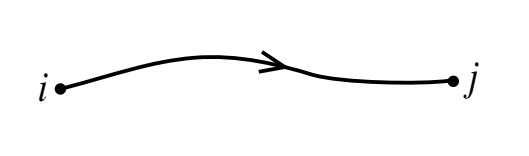
\includegraphics[width=0.5\textwidth]{figure/Fig6.4.jpg}\\
		\caption{An open string with Chan-Paton degrees of freedom .}\label{fig:6.4}
	\end{center}
\end{figure}

In the string theory of strong interactions, the motivation for introducing Chan-Paton factors was to introduce $SU(3)$ flavor quantum numbers: endpoints are like quarks and anti-quarks connected by a color-current tube . We now introduce it in a broader framework: consider all possible symmetries . In chapter \ref{cha:8}, we will give a new interpretation of Chan-Paton degrees of freedom, and in chapter 14, we will add a possible further improvement . Now there are $n^2$ scalar tachyons, $n^2$ massless vector bosons, and so on . Introduce $n^2$ Hermitian matrices $\lambda_{i j}^{a}$ and normalize as :
\begin{equation}
	\operatorname{Tr}(\lambda^{a} \lambda^{b})=\delta^{a b} \:, \label{6.5.2}
\end{equation}
These matrices are a complete basis for the states of the two endpoints . They are representation matrices of $U(n)$, so one can guess that the massless vector bosons are associated with $U(n)$ symmetry; we will soon see that this is indeed the case .

Define the basis :
\begin{equation}
	|N ; k ; a\rangle=\sum_{i, j=1}^{n}|N ; k ; i j\rangle \lambda_{i j}^{a}  \:. \label{6.5.3}
\end{equation}
Now consider the 4-tachyon amplitude shown in figure \ref{fig:6.2}(a), in which vertex operators are arranged in the cyclic order 1234 . Because Chan-Paton degrees of freedom do not appear in the Hamiltonian, their states cannot evolve between vertex operators: the state of the right endpoint of tachyon 1 must be the same as the state of the left endpoint of tachyon 2, and so on . Therefore, the amplitude in figure \ref{fig:6.2}(a) will contain the factor :
\begin{equation}
	\operatorname{Tr}(\lambda^{a_{1}} \lambda^{a_{2}} \lambda^{a_{3}} \lambda^{a_{4}}) \:, \label{6.5.4}
\end{equation}
which originates from the overlap of the Chan-Paton wavefunctions of each tachyon . This rule can be generalized to arbitrary amplitudes: each vertex operator now contains the Chan-Paton factor $\lambda_{i j}^{a}$ from the endpoint wavefunction, and the amplitude for each worldsheet is multiplied by the trace of Chan-Paton factors along the boundary . The 3-tachyon amplitude becomes :
\begin{align}
	S_{D_{2}}(k_{1}, a_{1} ; k_{2}, a_{2} ; k_{3}, a_{3})= 
	\frac{\mi g_{\mathrm{o}}}{\alpha^{\prime}}(2 \pi)^{26} \delta^{26}({\textstyle\sum_{i} k_{i}}) 
	\operatorname{Tr}(\lambda^{a_{1}} \lambda^{a_{2}} \lambda^{a_{3}}+\lambda^{a_{1}} \lambda^{a_{3}} \lambda^{a_{2}}) \:, \label{6.5.5}
\end{align}
The two cyclic orders now have different Chan-Paton traces . The 4-tachyon amplitude is :
\begin{align}
	&S_{D_{2}}(k_{1}, a_{1} ; k_{2}, a_{2} ; k_{3}, a_{3} ; k_{4}, a_{4})
	=\frac{\mi g_{\mathrm{o}}^{2}}{\alpha^{\prime}}(2 \pi)^{26} \delta^{26}({\textstyle \sum_{i} k_{i}}) \nonumber \\
	&\quad \times \Bigl[\operatorname{Tr}(\lambda^{a_{1}} \lambda^{a_{2}} \lambda^{a_{4}} \lambda^{a_{3}}
	+\lambda^{a_{1}} \lambda^{a_{3}} \lambda^{a_{4}} \lambda^{a_{2}}) B(-\alpha_{\mathrm{o}}(s),-\alpha_{\mathrm{o}}(t)) \nonumber  \\
	&\qquad+\operatorname{Tr}(\lambda^{a_{1}} \lambda^{a_{3}} \lambda^{a_{2}} \lambda^{a_{4}}
	+\lambda^{a_{1}} \lambda^{a_{4}} \lambda^{a_{2}} \lambda^{a_{3}}) B(-\alpha_{\mathrm{o}}(t),-\alpha_{\mathrm{o}}(u))\nonumber \\
	&\qquad+\operatorname{Tr}(\lambda^{a_{1}} \lambda^{a_{2}} \lambda^{a_{3}} \lambda^{a_{4}}
	+\lambda^{a_{1}} \lambda^{a_{4}} \lambda^{a_{3}} \lambda^{a_{2}}) 
	B(-\alpha_{\mathrm{o}}(s),-\alpha_{\mathrm{o}}(u))\Bigr] \:. \label{6.5.6}
\end{align}
Again considering the unitarity relation \eqref{6.4.13}, the pole at $s=-1 / \alpha^{\prime}$ gives the left side the factor :
\begin{equation}
	\frac{1}{4} \operatorname{Tr}\Bigl(\{\lambda^{a_{1}}, \lambda^{a_{2}}\} \{\lambda^{a_{3}}, \lambda^{a_{4}}\}\Bigr) \:,\label{6.5.7}
\end{equation}
while the right side gains the factor :
\begin{equation}
	\frac{1}{4} \sum_{a} \operatorname{Tr}\Bigl(\{\lambda^{a_{1}}, \lambda^{a_{2}}\} \lambda^{a}\Bigr) 
	\operatorname{Tr}\Bigl(\{\lambda^{a_{3}}, \lambda^{a_{4}}\} \lambda^{a}\Bigr) \:, \label{6.5.8}
\end{equation}
namely summing over the Chan-Paton wavefunctions of the intermediate states . The completeness and normalization \eqref{6.5.2} of $\lambda_{i j}^{a}$ imply that for any $A$ and $B$, one has :
\begin{equation}
	\operatorname{Tr}(A \lambda^{a}) \operatorname{Tr}(B \lambda^{a})=\operatorname{Tr}(A B) \:,  \label{6.5.9}
\end{equation}
thus the amplitude remains unitary .
\begin{tcolorbox}
	\begin{proof}
		Let $\operatorname{Tr}(A \lambda^{a})=\langle A \vert \lambda^{a}\rangle=\langle\lambda^{a}|A\rangle$, then :
		\[
		\operatorname{Tr}(A \lambda^{a}) \operatorname{Tr}(B \lambda^{a}) = 
		\langle A \vert \lambda^{a}\rangle\langle\lambda^{\alpha} \vert B\rangle=\langle A \vert B\rangle \:,
		\]
		where $\sum_{a}|\lambda^{a}\rangle\langle\lambda^{a}|=1$ comes from $\langle\lambda^{a} \vert \lambda^{b}\rangle= \delta^{a b}$ .
	\end{proof}	
\end{tcolorbox}



\subsection*{Gauge Interactions}
The amplitude of a gauge boson with two tachyons is :
\begin{align}
	&S_{D_{2}}(k_{1}, a_{1}, e_{1} ; k_{2}, a_{2} ; k_{3}, a_{3})= 
	-\mi g_{\mathrm{o}}^{\prime} g_{\mathrm{o}}^{2} \me^{-\lambda} e_{1 \mu} \nonumber \\
	&\quad \times\Bigl\langle \bno c^{1} \dot{X}^{\mu} \me^{\mi k_{1} \cdot X}(y_{1})\bno 
	\bno  c^{1} \me^{\mi k_{2} \cdot X}(y_{2})\bno \bno c^{1} \me^{\mi k_{3} \cdot X}(y_{3})\bno\Bigr\rangle_{D_{2}} 
	\operatorname{Tr}(\lambda^{a_{1}} \lambda^{a_{2}} \lambda^{a_{3}})  \nonumber\\
	&\qquad \qquad +(k_{2}, a_{2}) \leftrightarrow(k_{3}, a_{3}) \:. \label{6.5.10}
\end{align}
We use the bosonic vertex operator \eqref{3.6.26}, but temporarily allow an independent normalization constant $g_{\mathrm{o}}^{\prime}$ . Using the results from section \ref{sec:6.2}, the path integral of $X$ is :
\begin{align}
	&\Bigl\langle \bno \dot{X}^{\mu} \me^{\mi k_{1} \cdot X}(y_{1})\bno \bno \me^{\mi k_{2} \cdot X}(y_{2})\bno 
	\bno \me^{\mi k_{3} \cdot X}(y_{3})\bno \Bigr\rangle_{D_{2}} 
	=-2 \mi \alpha^{\prime}\biggl(\frac{k_{2}^{\mu}}{y_{12}}+\frac{k_{3}^{\mu}}{y_{13}}\biggr) \nonumber \\
	&\qquad \times \mi C_{D_{2}}^{X}(2 \pi)^{26} \delta^{26}({\textstyle \sum_{i} k_{i}})
	|y_{12}|^{2 \alpha^{\prime} k_{1} \cdot k_{2}}|y_{13}|^{2 \alpha^{\prime} k_{1} \cdot k_{3}} 
	|y_{23}|^{2 \alpha^{\prime} k_{2} \cdot k_{3}} \:. \label{6.5.11}
\end{align}
Using momentum conservation, mass-shell condition, and physical state condition $k_{1} \cdot e_{1}=0$, the amplitude becomes :
\begin{align}
	&S_{D_{2}}(k_{1}, a_{1}, e_{1} ; k_{2}, a_{2} ; k_{3}, a_{3}) \nonumber \\
	&=-\mi g_{\mathrm{o}}^{\prime} e_{1} \cdot k_{23}(2 \pi)^{26} \delta^{26}({\textstyle \sum_{i} k_{i}}) 
	\operatorname{Tr}\Bigl(\lambda^{a_{1}}[\lambda^{a_{2}}, \lambda^{a_{3}}]\Bigr) \:, \label{6.5.12}
\end{align}
where $k_{i j} \equiv k_{i}-k_{j}$ . This is again independent of the position of vertex operators .

The $s=0$ pole in the 4-tachyon amplitude is no longer zero . The term that was canceled now has Chan-Paton factors in a different order, so the pole is proportional to :
\begin{equation}
	\operatorname{Tr}\Bigl([\lambda^{a_{1}}, \lambda^{a_{2}}][\lambda^{a_{3}}, \lambda^{a_{4}}]\Bigr) \:. \label{6.5.13}
\end{equation}
Relating the coefficient of this pole to the amplitude \eqref{6.5.12} through unitarity gives :
\begin{equation}
	g_{\mathrm{o}}^{\prime}=(2 \alpha^{\prime})^{-1 / 2} g_{\mathrm{o}} \:. \label{6.5.14}
\end{equation}
This is the same as the relative normalization derived from the state-operator map: there is only one independent coupling constant . For the coupling of 3 gauge bosons, a similar calculation gives :
\begin{align}
	&S_{D_{2}}(k_{1}, a_{1}, e_{1} ; k_{2}, a_{2}, e_{2} ; k_{3}, a_{3}, e_{3}) \nonumber \\
	&\qquad = \mi g_{\mathrm{o}}^{\prime}(2 \pi)^{26} \delta^{26}({\textstyle\sum_{i} k_{i}})
	\Bigl(e_{1} \cdot k_{23} e_{2} \cdot e_{3}+e_{2} \cdot k_{31} e_{3} \cdot e_{1}+e_{3} \cdot k_{12} e_{1} \cdot e_{2} \nonumber\\
	&\qquad \qquad +\frac{\alpha^{\prime}}{2} e_{1} \cdot k_{23} e_{2} \cdot k_{31} e_{3} \cdot k_{12} \Bigr) 
	\operatorname{Tr}\Bigl(\lambda^{a_{1}}[\lambda^{a_{2}}, \lambda^{a_{3}}]\Bigr) \:. \label{6.5.15}
\end{align}

To first order in momentum, the amplitudes we found can be re-produced from the following spacetime action :
\begin{equation}
	\bm{S}=\frac{1}{g_{\mathrm{o}}^{\prime 2}} \int \dif^{26} x\: \biggl[-\frac{1}{2} \operatorname{Tr}(D_{\mu} \varphi D^{\mu}\varphi)+\frac{1}{2 \alpha^{\prime}} \operatorname{Tr}(\varphi^{2})+\frac{2^{1 / 2}}{3 \alpha^{\prime 1 / 2}} 
	\operatorname{Tr}(\varphi^{3})
	-\frac{1}{4} \operatorname{Tr}(F_{\mu \nu} F^{\mu \nu})\biggr] \:, \label{6.5.16}
\end{equation}
where the tachyon field $\varphi$ and the Yang-Mills vector potential $A_{\mu}$ are written as $n \times n$ matrices, i.e., $A_{\mu}=A_{\mu}^{a} \lambda^{a}$ . Furthermore, $D_{\mu} \varphi=\partial_{\mu} \varphi-\mi[A_{\mu}, \varphi]$, and $F_{\mu \nu}=\partial_{\mu} A_{\nu}-\partial_{\nu} A_{\mu}-\mi[A_{\mu}, A_{\nu}]$ .

This is the action for a $U(n)$ gauge field coupled to a scalar field in the adjoint representation . The addition of the Chan-Paton factor is exactly what is needed for the gauge-invariant representation . Since decoupling of non-physical states is guaranteed in string perturbation theory, gauge invariance is automatic, and we will study it further .

At momentum $k$ much smaller than the string scale, the only open string state is the massless gauge boson . As discussed in section \ref{sec:3.7}, in this limit, the physics should reduce to an effective field theory of massless states . Therefore, introducing the tachyon into the action \eqref{6.5.16} must be illogical in some places; we did so for heuristics . But now let us focus on the gauge boson . The form of the 4-gauge boson amplitude is similar to the Veneziano amplitude, but with extra structure from the polarization tensor . Expanding it as a power series in $\alpha^{\prime} k^{2}$, the first term survives in the zero-slope limit; it is the sum of pole terms in $s, t, u$ plus a constant . Consistency will guarantee that it is exactly the same as the 4-gauge boson amplitude obtained from the Yang-Mills Lagrangian $F_{\mu \nu} F^{\mu\nu}$ in field theory . Note, however, the term at order $\alpha^{\prime} k^{3}$ in the 3-gauge boson amplitude \eqref{6.5.15} . This implies higher-order derivative terms in the Lagrangian :
\begin{equation}
	-\frac{2 \mi \alpha^{\prime}}{3 g_{\text{o}}^{\prime 2}} \operatorname{Tr}(F_{\mu}{}^{\nu} F_{\nu}{}^{\omega} F_{\omega}{}^{\mu}) \:. \label{6.5.17}
\end{equation}
Similarly, expanding the 4-point amplitude will reveal an infinite sum of high-order interaction terms (besides \eqref{6.5.17}, they indeed have no kinematic contribution to the 3-gauge boson amplitude) . In low-energy regions, string loop amplitudes also reduce to loops obtained from the effective Lagrangian . By the general logic of effective Lagrangians, higher-order derivative terms are not very important at low energies  ; they become important at the scale $\alpha^{\prime} k^{2} \approx 1$, which is where new physics (massive string states) appears and the effective action is no longer applicable .

If we have a cutoff, why do we still need renormalization? Renormalization still has meaning . And in fact, this is its true interpretation: it means that low-energy physics is independent of the details of high-energy physics, except for the parameters in the effective Lagrangian . This is bittersweet: it means we can use ordinary quantum field theory to make predictions at accelerator energy levels without knowing the theory at the Planck scale, but it also means we cannot use physics at particle accelerators to probe the theory at the Planck scale .

String spectra and amplitudes have an obvious global $U(n)$ symmetry ,
\begin{equation}
	\lambda^{a} \rightarrow U \lambda^{a} U^{\dagger} \:, \label{6.5.18}
\end{equation}
which preserves the Chan-Paton trace and the norm of the states . From the details of the amplitudes, we see that this is actually local symmetry of spacetime . We will see that the elevation from global worldsheet symmetry to local spacetime symmetry is a very common phenomenon in string theory .

All open string states transform according to the $n \times n$ adjoint representation under $U(n)$ symmetry . Incidentally, $U(n)$ is not a simple Lie algebra: $U(n)=SU(n) \times U(1)$ . The $U(1)$ gauge boson, $\lambda_{i j}=\delta_{i j} / n^{1 / 2}$, decouples from amplitudes \eqref{6.5.12} and \eqref{6.5.15} . The adjoint representation of $U(1)$ is trivial, so all string states are neutral under $U(1)$ symmetry .

\subsection*{Non-orientable Strings}

The extension to non-orientable strings is interesting . First consider a theory without Chan-Paton factors . Besides Möbius invariance, the $X^{\mu}$ CFT on a sphere or disk is invariant under reflection symmetry in the direction of the open string $\sigma^{1} \rightarrow \pi-\sigma^{1}$ or on a closed string $\sigma^{1} \rightarrow 2 \pi-\sigma^{1}$ . Worldsheet parity is generated by the operator $\Omega$ . From the mode expansion, in open strings :
\begin{equation}
	\Omega \alpha_{n}^{\mu} \Omega^{-1}=(-1)^{n} \alpha_{n}^{\mu} \:, \label{6.5.19}
\end{equation}
and in closed strings :
\begin{equation}
	\Omega \alpha_{n}^{\mu} \Omega^{-1}=\tilde{\alpha}_{n}^{\mu} \:. \label{6.5.20}
\end{equation}
This symmetry also extends to ghost fields . But for concentration, we do not discuss them here; their contribution to tree-level diagrams is merely a fixed factor .

Regardless of whether it is an open or closed string, tachyon vertex operators are even under worldsheet parity (this is obvious for ghost-free integrated vertex operators; fixed operators must transform in the same way), which determines the sign of the operator . Then all states can be categorized according to their parity eigenvalues $\omega=\pm 1$ . The relation \eqref{6.5.19} in open strings implies :
\begin{equation}
	\Omega|N ; k\rangle=\omega_{N}|N ; k\rangle, \quad \omega_{N}=(-1)^{1+\alpha^{\prime} m^{2}} \:. \label{6.5.21}
\end{equation}
Worldsheet parity is multiplicative conservation . For example, the 3-tachyon amplitude is non-zero, consistent with $(+1)^{3}=1$ . On the other hand, massless vectors have $\omega=-1$, so we can expect the vector-tachyon-tachyon amplitude \eqref{6.5.10} and the 3-vector amplitude \eqref{6.5.15} to be zero in the absence of Chan-Paton factors, and this is indeed the case ($\lambda^{a}$ is replaced by 1, and the commutator is zero) . Different cyclic orders are also related to each other via worldsheet parity and thus cancel out .

Given a consistent oriented string theory, by restricting the spectrum to states with $\omega=+1$, we give a new non-orientable string theory . States where $\alpha^{\prime} m^{2}$ is odd are retained, while states where $\alpha^{\prime} m^{2}$ is even, including the photon, are forbidden . $\omega$ conservation guarantees that if all external states have $\omega=+1$, then intermediate states of tree-level diagrams also have $\omega=+1$ . Therefore, at least at the tree level, the unitarity of non-orientable strings follows from the unitarity of oriented strings .

The primary interest in non-orientable theory lies in the treatment of Chan-Paton factors . Since we can identify opposite endpoints of an open string, worldsheet parity must reverse them :
\begin{equation}
	\Omega|N ; k ; i j\rangle=\omega_{N}|N ; k ; j i\rangle \:. \label{6.5.22}
\end{equation}
Once again, this is a symmetry of all amplitudes in the oriented theory . To form a non-orientable theory, we again constrain the spectrum to worldsheet parity eigenvalues $\omega=+1$ . Take a set of basis for $\lambda_{i j}^{a}$ such that each matrix is either symmetric $s^{a}=+1$ or antisymmetric $s^{a}=-1$ . Then :
\begin{equation}
	\Omega|N ; k ; a\rangle=\omega_{N} s^{a}|N ; k ; a\rangle \:. \label{6.5.23}
\end{equation}
The worldsheet parity eigenvalue is $\omega=\omega_{N} s^{a}$, so the non-orientable spectrum is :
\begin{subequations} \label{6.5.24}
	\begin{align}
		&\text{even multiples of } \alpha^{\prime} m^{2} \:: \qquad   \text{antisymmetric } \lambda^{a}  \:, \label{6.5.24a} \\ 	
		&\text{odd multiples of } \alpha^{\prime} m^{2} \:: \qquad   \text{symmetric } \lambda^{a}  \:. \label{6.5.24b} 
	\end{align}			
\end{subequations}
For massless gauge bosons, Chan-Paton factors are $n \times n$ antisymmetric matrices, so the gauge group is $SO(n)$ . States at even mass levels transform according to the adjoint representation of the orthogonal group $SO(n)$, while states at odd mass levels transform according to a traceless symmetric tensor plus a singlet representation . The oriented theory has a large class of direction-reversing symmetries obtained as a combination of $\Omega$ and $U(n)$ rotations :
\begin{equation}
	\Omega_{\gamma}|N ; k ; i j\rangle=\omega_{N} \gamma_{j j^{\prime}}\left|N ; k ; j^{\prime} i^{\prime}\right\rangle \gamma_{i^{\prime} i}^{-1} \:. \label{6.5.25}
\end{equation}
By restricting the spectrum to $\omega_{y}=+1$, we can construct more general non-orientable theories . This is again compatible with interactions; applying $\Omega_{\gamma}$ twice gives :
\begin{equation}
	\Omega_{\gamma}^{2}|N ; k ; i j\rangle= [(\gamma^{T})^{-1} \gamma]_{i i^{\prime}} |N ; k ; i^{\prime} j^{\prime}\rangle (\gamma^{-1} \gamma^{T})_{j^{\prime} j} \:. \label{6.5.26}
\end{equation}
We assume $\Omega_{\gamma}^{2}=1$ for reasons explained below . This implies :
\begin{equation}
	\gamma^{T}=\pm \gamma \:. \label{6.5.27}
\end{equation}
That is, $\gamma$ is symmetric or antisymmetric .

The Chan-Paton basis transformation is :
\begin{equation}
	|N ; k ; i j\rangle^{\prime}=U_{i i^{\prime}}^{-1} |N ; k ; i^{\prime} j^{\prime}\rangle U_{j^{\prime} j} \:, \label{6.5.28}
\end{equation}
which changes $\gamma$ to :
\begin{equation}
	\gamma^{\prime}=U^{T} \gamma U \:. \label{6.5.29}
\end{equation}
In the symmetric case, one can always find a basis such that $\gamma=1$, which gives the case already examined above . In the antisymmetric case, there exists a basis such that :
\begin{equation}
	\gamma=M \equiv \mi\begin{bmatrix}
		0 & I \\
		-I & 0
	\end{bmatrix} \:. \label{6.5.30}
\end{equation}
Here $I$ is a $k \times k$ identity matrix; since $\gamma$ is an invertible antisymmetric matrix, $n=2 k$ must be even . We take a basis for the Chan-Paton wavefunctions such that $M(\lambda^{a})^{T} M=s^{a^{\prime}} \lambda^{a}$, where $s^{a^{\prime}}=\pm 1$ . Then the worldsheet eigenvalue is $\omega_{\gamma}=\omega_{N} s^{a^{\prime}}$, and the non-orientable spectrum is :
\begin{subequations} \label{6.5.31}
	\begin{align}
		\text{even multiples of } \alpha^{\prime} m^{2} \:: \qquad   M(\lambda^{a})^{T} M=-\lambda^{a} \:, \label{6.5.31a} \\
		\text{odd multiples of } \alpha^{\prime} m^{2} \:: \qquad   M(\lambda^{a})^{T} M=+\lambda^{a} \:. \label{6.5.31b}
	\end{align}
\end{subequations}
At even mass levels, including gauge bosons, this defines the adjoint representation of the symplectic group $Sp(k)$ .

To construct a non-orientable theory, we must have $\Omega_{\gamma}^{2}=1$ for the following reasons . Since $\Omega^{2}=1$, $\Omega_{\gamma}^{2}$ must only act on the Chan-Paton factors . In fact, from \eqref{6.5.26}, its action on the Chan-Paton wavefunction is :
\begin{equation}
	\lambda \rightarrow (\gamma^{T})^{-1} \gamma \lambda \gamma^{-1} \gamma^{T}=\lambda \:, \label{6.5.32}
\end{equation}
where, since all states are invariant under $\Omega_{\gamma}$, the last equal sign must hold in non-orientable theory . Now we assert that the allowed Chan-Paton wavefunctions must constitute a complete basis . The key is that two open strings can exchange endpoints through the split-aggregate interaction in figure \ref{fig:3.4}(c) . In this way, a complete basis, namely any Chan-Paton state $|i j\rangle$, can be reached . By Schur's Lemma, if \eqref{6.5.32} holds for the complete basis, then $\gamma^{-1} \gamma^{T}=1$, hence $\Omega_{\gamma}^{2}=1$ . By taking different sets of $\lambda^{a}$, we can try to obtain different gauge theories . In fact, the oriented $U(n)$ theory and non-orientable $SO(n)$ and $Sp(k)$ theories constructed above are the only possibilities . The extension of the completeness discussion in \eqref{6.5.7} -- \eqref{6.5.9} shows they are the most general solutions for non-orientable theories . In particular, exceptional Lie algebras cannot be obtained from Chan-Paton factors . In closed string theory, there are other mechanisms giving gauge bosons and allowing other groups .

\section{Closed string tree amplitudes} \label{sec:6.6}

The discussion of closed string amplitudes is similar to the above . The amplitude of 3 closed string tachyons is :
\begin{equation}
	S_{S_{2}}(k_{1} ; k_{2} ; k_{3})=g_{\mathrm{c}}^{3} \me^{-2 \lambda}\left\langle\prod_{i=1}^{3} : \mathrel{\tilde{c} c \me^{\mi k_{i} \cdot X}(z_{i}, \bar{z}_{i})}:\right\rangle \bigg._{\!\!S_{2}} \:. \label{6.6.1}
\end{equation}
In this case, the CKG $PSL(2, \mathds{C})$ (Möbius group) can fix three vertex operators at arbitrary positions $z_{1,2,3}$ . Taking the expectation value from section \ref{sec:6.2}, the result is again independent of the vertex operators :
\begin{equation}
	S_{S_{2}}(k_{1} ; k_{2} ; k_{3})= \mi g_{\mathrm{c}}^{3} C_{S_{2}}(2 \pi)^{26} \delta^{26}({\textstyle \sum_{i} k_{i}}) \:, \label{6.6.2}
\end{equation}
where $C_{S_{2}}=\me^{-2 \lambda} C_{S_{2}}^{X} C_{S_{2}}^{\mathrm{g}}$ .

For 4 closed string tachyons :
\begin{equation}
	S_{S_{2}}(k_{1} ; k_{2} ; k_{3} ; k_{4})=g_{\mathrm{c}}^{4} \me^{-2 \lambda} 
	\int_{\mathds{C}} \dif^{2} z_{4} \: \left\langle\prod_{i=1}^{3}
	: \mathrel{\tilde{c} c \me^{\mi k_{i} \cdot X}(z_{i}, \bar{z}_{i})}:
	: \mathrel{\me^{\mi k_{4} \cdot X}(z_{4}, \bar{z}_{4})}:\right\rangle\bigg._{\!\!S_{2}} \:, \label{6.6.3}
\end{equation}
where the integral range is the entire complex plane $\mathds{C}$ . Calculating the expectation value and letting $z_{1}=0, z_{2}=1, z_{3}=\infty$, this becomes :
\begin{equation}
	S_{S_{2}}(k_{1} ; k_{2} ; k_{3} ; k_{4}) = 
	\mi g_{\mathrm{c}}^{4} C_{S_{2}}(2 \pi)^{26} \delta^{26}({\textstyle\sum_{i} k_{i}}) J(s, t, u) \:, \label{6.6.4}
\end{equation}
where :
\begin{equation}
	J(s, t, u)=\int_{\mathds{C}} \dif^{2} z_{4}\: |z_{4}|^{-\alpha^{\prime} u / 2-4}|1-z_{4}|^{-\alpha^{\prime} t/2-4}\:. \label{6.6.5}
\end{equation}
Here $s+t+u=-16 / \alpha^{\prime}$; we have labeled here the correlation of $J$ with all 3 variables to emphasize their symmetry . When $s, t, u<-4 / \alpha^{\prime}$, the amplitude converges . As $z_{4} \rightarrow 0$, it has a pole with respect to $u$; as $z_{4} \rightarrow 1$, it has a pole with respect to $t$; as $z_{4} \rightarrow \infty$, it has a pole with respect to $s$ . These poles are at :
\begin{equation}
	\alpha^{\prime} s\,,\: \alpha^{\prime} t \,,\: \alpha^{\prime} u=-4,0,4,8, \ldots,\label{6.6.6}
\end{equation}
which are the mass squared of closed string states . The pole at $\alpha^{\prime} s=-4$ is :
\begin{equation}
	\mi g_{\mathrm{c}}^{4} C_{S_{2}} \int_{|z_{4}|>1 / \epsilon} \dif^{2} z_{4}\: |z_{4}|^{\alpha^{\prime} s / 2} 
	\sim-\frac{8 \pi \mi g_{\mathrm{c}}^{4} C_{S_{2}}}{\alpha^{\prime} s+4} \:. \label{6.6.7}
\end{equation}
Unitarity gives :
\begin{equation}
	C_{S_{2}}=\frac{8 \pi}{\alpha^{\prime} g_{\mathrm{c}}^{2}} \:, \label{6.6.8}
\end{equation}
therefore :
\begin{equation}
	S_{S_{2}}(k_{1} ; k_{2} ; k_{3})=\frac{8 \pi \mi g_{\mathrm{c}}}{\alpha^{\prime}}(2 \pi)^{26} 
	\delta^{26}({\textstyle\sum_{i} k_{i}}) \:. \label{6.6.9}
\end{equation}

Similar to the Veneziano amplitude, the 4-closed-string-tachyon amplitude can be expressed as gamma functions :
\begin{equation}
	S_{S_{2}}(k_{1} ; k_{2} ; k_{3} ; k_{4})=\frac{8 \pi \mi g_{\mathrm{c}}^{2}}{\alpha^{\prime}}(2 \pi)^{26} 
	\delta^{26}({\textstyle \sum_{i} k_{i}}) C(-\alpha_{\mathrm{c}}(t),-\alpha_{\mathrm{c}}(u)) \:, \label{6.6.10}
\end{equation}
where $\alpha_{\mathrm{c}}(x)=1+\alpha^{\prime} x / 4$ and :
\begin{align}
	C(a, b) &=\int_{\mathds{C}} \dif^{2} z \: |z|^{2 a-2}|1-z|^{2 b-2} \nonumber \\
	&=2 \pi \frac{\Gamma(a) \Gamma(b) \Gamma(c)}{\Gamma(a+b) \Gamma(a+c) \Gamma(b+c)}\:, \quad a+b+c=1 \:. \label{6.6.11}
\end{align}
This is the Virasoro-Shapiro amplitude . There is only one term, and the poles in the $s, t, u$ channels come from the gamma functions in the numerator . Similar to the Veneziano amplitude, the Virasoro-Shapiro amplitude exhibits Regge behavior in the Regge limit :
\begin{equation}
	S_{S_{2}}(k_{1} ; k_{2} ; k_{3} ; k_{4}) \propto s^{2 \alpha_{\mathrm{c}}(t)} 
	\frac{\Gamma(-\alpha_{\mathrm{c}}(t))}{\Gamma(1+\alpha_{\mathrm{c}}(t))} \:, \label{6.6.12}
\end{equation}
and exponential behavior in the hard scattering limit :
\begin{equation}
	S_{S_{2}}(k_{1} ; k_{2} ; k_{3} ; k_{4}) \propto \exp 
	\biggl[-\frac{\alpha^{\prime}}{2}(s \ln s \alpha^{\prime}+t \ln t \alpha^{\prime}+u \ln u \alpha^{\prime})\biggr] \:. \label{6.6.13}
\end{equation}

On the sphere, the amplitude for one massless closed string and two closed string tachyons is :
\begin{align}
	S_{S_{2}}(k_{1}, e_{1} ; k_{2} ; k_{3}) &= g_{\mathrm{c}}^{2} g_{\mathrm{c}}^{\prime} 
	\me^{-2 \lambda} e_{1 \mu \nu} \Biggl\langle: \mathrel{\tilde{c} c \partial X^{\mu} \bar{\partial} X^{\nu} 
		\me^{\mi k_{1} \cdot X}(z_{1}, \bar{z}_{1})}: \nonumber \\
	&\qquad \qquad \quad : \mathrel{\tilde{c} c \me^{\mi k_{2} \cdot X}(z_{2}, \bar{z}_{2})}:
	: \mathrel{\tilde{c} c \me^{\mi k_{3} \cdot X}(z_{3}, \bar{z}_{3})}: \biggr\rangle_{S_{2}}  \nonumber \\
	& =-\frac{\pi \mi \alpha^{\prime}}{2} g_{\mathrm{c}}^{\prime} e_{1 \mu \nu} k_{23}^{\mu} k_{23}^{\nu}
	(2 \pi)^{26} \delta^{26}({\textstyle\sum_{i} k_{i}}) \:, \label{6.6.14}
\end{align}
where $e_{1 \mu \nu} e_{1}^{\mu \nu}=1$ . Expanding the Virasoro-Shapiro amplitude \eqref{6.6.10} at the $s=0$ pole, unitarity can give :
\begin{equation}
	g_{\mathrm{c}}^{\prime}=\frac{2}{\alpha^{\prime}} g_{\mathrm{c}} \:, \label{6.6.15}
\end{equation}
which is again consistent with the state-operator map containing the overall constant $g_{\mathrm{c}}$ . The amplitude \eqref{6.6.14} can be obtained from field theory via the action $\bm{S}+\bm{S}_{T}$, where $\bm{S}$ is the action for massless fields \eqref{3.7.20}, and :
\begin{equation}
	\bm{S}_{T}=-\frac{1}{2} \int \dif^{26} x\: (-G)^{1 / 2} \me^{-2 \tilde{\Phi}}
	\biggl(G^{\mu \nu} \partial_{\mu} T \partial_{\nu} T-\frac{4}{\alpha^{\prime}} T^{2} \biggr) \:, \label{6.6.16}
\end{equation}
which is the action for a closed string tachyon $T$ . For example, the graviton amplitude with polarization $e_{\mu \nu}$ can be obtained by expanding :
\begin{equation}
	\tilde{G}_{\mu \nu}=\eta_{\mu \nu}-2 \kappa e_{\mu \nu} \me^{\mi k \cdot x} \:, \label{6.6.17}
\end{equation}
from this action . Note that this is the Einstein metric, and its action \eqref{3.7.25} does not contain the dilaton . The normalization of the fluctuation is determined by the fluctuation of the graviton kinetic energy term in the spacetime action . Specifically, if taking $\tilde{G}_{\mu \nu}-\eta_{\mu \nu}=-2 \kappa e_{\mu \nu} f(x)$ where $e_{\mu \nu} e^{\mu \nu}=1$, the effective action of $f$ has the canonical normalization $\frac{1}{2}$ for real scalars . The field theory amplitude matches the string theory result \eqref{6.6.14} and relates to the normalization of the gravitational coupling vertex operator :
\begin{equation}
	\kappa=\pi \alpha^{\prime} g_{\mathrm{c}}^{\prime}=2 \pi g_{\mathrm{c}} \:. \label{6.6.18}
\end{equation}

The 3-massless-closed-string amplitude is :
\begin{equation}
	S_{S_{2}}(k_{1}, e_{1} ; k_{2}, e_{2} ; k_{3}, e_{3})=\frac{\mi \kappa}{2}(2 \pi)^{26} 
	\delta^{26}(\textstyle{\sum_{i} k_{i}}) e_{1 \mu \nu} e_{2 \alpha \beta} e_{3 \gamma \delta} T^{\mu \alpha \gamma} T^{\nu \beta \delta} \:, \label{6.6.19}
\end{equation}
where :
\begin{equation}
	T^{\mu \alpha \gamma}=k_{23}^{\mu} \eta^{\alpha \gamma}+k_{31}^{\alpha} \eta^{\gamma \mu}+k_{12}^{\gamma} \eta^{\mu \alpha}+\frac{\alpha^{\prime}}{8} k_{23}^{\mu} k_{31}^{\alpha} k_{12}^{\gamma} \:. \label{6.6.20}
\end{equation}
The $k^2$ term of this amplitude corresponds to the spacetime action \eqref{3.7.25}, while the $k^4$ and $k^6$ terms come from several high-order derivative interactions, including terms of order 2 and 3 in the spacetime curvature . Higher-order corrections to the action can also be obtained by calculating high-loop corrections of the worldsheet $\beta$ function \eqref{3.7.14} .

If we set $\alpha^{\prime}=\frac{1}{2}$ for open strings and $\alpha^{\prime}=2$ for closed strings, the tensor structure of the closed string amplitude \eqref{6.6.19} is just two copies of the open string amplitude \eqref{6.5.15} . The same result holds for the amplitude \eqref{6.6.14} . This is the result of the free-field expectation values on the sphere factorizing into holomorphic and anti-holomorphic parts . Similar factorization occurs for four or more closed strings before integrating over the vertex operator positions . Furthermore, through careful treatment of the integration contours, it is possible to find relations between the integrated amplitudes . For 4-tachyon amplitudes, after using $\Gamma(x) \Gamma(1-x) \sin (\pi x)=\pi$, the above integrals have the following relationship :
\begin{equation}
	J(s, t, u, \alpha^{\prime})=-2 \sin \pi \alpha_{\mathrm{c}}(t) I(s, t, 4 \alpha^{\prime}) I(t, u, 4 \alpha^{\prime}) \:; \label{6.6.21}
\end{equation}
we have now indicated the explicit correlation of the integral for $\alpha^{\prime}$ . For the general integral appearing in 4-point closed string amplitudes, there is the following relationship :
\begin{align}
	&\int_{\mathds{C}} \dif^{2} z\: z^{a-1+m_{1}} \bar{z}^{a-1+n_{1}}(1-z)^{b-1+m_{2}}(1-\bar{z})^{b-1+n_{2}} \nonumber \\
	&\qquad =2 \sin [\pi(b+n_{2})] B(a+m_{1}, b+m_{2}) B(b+n_{2}, 1-a-b-n_{1}-n_{2}) \:. \label{6.6.22}
\end{align}
This implies the relationship between 4-point open string amplitudes and 4-point closed string amplitudes :
\begin{equation}
	A_{\mathrm{c}}(s, t, u, \alpha^{\prime}, g_{\mathrm{c}}) = 
	\frac{\pi \mi g_{\mathrm{c}}^{2} \alpha^{\prime}}{g_{\mathrm{o}}^{4}} 
	\sin [\pi \alpha_{\mathrm{c}}(t)] A_{\mathrm{o}}(s, t, \tfrac{1}{4} \alpha^{\prime}, g_{\mathrm{o}}) 
	A_{\mathrm{o}}(t, u, \tfrac{1}{4} \alpha^{\prime}, g_{\mathrm{o}})^{*} \:, \label{6.6.23}
\end{equation}
where the open string amplitude contains only one of the 6 cyclic orderings, and the pole is in the stated channel .

\subsection*{Consistency}
In chapter \ref{cha:9}, we will discuss convergence and gauge invariance of tree-level amplitudes in a general way, but as an introduction, we now first use OPE to see how this works at the lowest order . Examine the operator product :
\begin{align}
	&: \mathrel{\me^{\mi k_{1} \cdot X(z_{1}, \bar{z}_{1})}}: 
	: \mathrel{\me^{\mi k_{4} \cdot X(z_{4}, \bar{z}_{4})}}: = 
	|z_{14}|^{\alpha^{\prime} k_{1} \cdot k_{4}}:\!\!
	\Bigl(1+ \mi z_{14} k_{1} \cdot \partial X + \mi \bar{z}_{14} k_{1} \cdot \bar{\partial} X \nonumber \\
	&\qquad \qquad -z_{14} \bar{z}_{14} k_{1} \cdot \partial X k_{1} \cdot \bar{\partial} X+\cdots \Bigr) 
	\,\me^{\mi(k_{1}+k_{4}) \cdot X}(z_{4}, \bar{z}_{4})\!\!: \:. \label{6.6.24}
\end{align}
It appears in amplitudes where $z_{14}$ is integrated out . When :
\begin{equation}
	\alpha^{\prime} k_{1} \cdot k_{4}=\frac{\alpha^{\prime}}{2}(k_{1}+k_{4})^{2}-4>-2 \:, \label{6.6.25}
\end{equation}
the integral converges at $z_{14} \rightarrow 0$, and it has a pole at $-2$ . The coefficient of this pole is the tachyon vertex operator . Therefore, in any amplitude, if a pair of tachyons has total momentum $(k_{1}+k_{4})^{2}=4 / \alpha^{\prime}$, there will be a pole, and unitarity requires this pole to be proportional to the amplitude with one fewer tachyon . Poles in momentum space correspond to long distances in spacetime, so this is a process where two tachyons scatter into one tachyon, which then interacts with other particles . Further doing OPE, the $O(z_{14})$ and $O(\bar{z}_{14})$ terms do not produce tachyons because the angular integration gives zero residue, and $O(z_{14} \bar{z}_{14})$ gives massless poles, and so on . Now we study more closely how local spacetime symmetry is maintained in string amplitudes . If any polarization vector is of the form $e_{\mu}=k_{\mu}$, or $e_{\mu \nu}=\zeta_{\mu} k_{\nu}+k_{\mu} \tilde{\zeta}_{\mu}$, where $k \cdot \zeta=k \cdot \tilde{\zeta}=0$, the scattering amplitudes we calculated are all zero . This corresponds to the action being invariant under Yang-Mills, coordinate, and antisymmetric tensor symmetries . As discussed in section \ref{sec:3.6}, the vertex operator of longitudinal polarization is the sum of a full derivative and another term, which is zero due to the equations of motion . After integration, the full derivative term is zero, but the equations of motion term may have sources at other vertex locations in the path integral . When $k_{1} \cdot k_{4}$ is large, the operator product \eqref{6.6.24} decreases rapidly to zero . Using this property, for any pair of operators, there will always be a kinematic region where all possible connected terms (contact) are suppressed . Then the amplitude of null polarization is identically zero in this region because all amplitudes except at poles are analytic; the amplitude of null polarization must be zero everywhere . We see that the poles required by unitarity and the destruction of all possible divergences and spacetime gauge invariance arise in the limits $z \rightarrow 0,1, \infty$ and when two vertex operators approach each other . For a sphere with 4 marked points, they are the boundaries of the moduli space . For historical reasons, the analytic continuation discussion here is called the canceled propagator argument .

\subsection*{Closed Strings on $D_{2}$ and $RP_{2}$}
Lowest-order closed-string-open-string interactions come from disks having both closed string vertex operators and open string vertex operators . Their low-energy effective actions can be derived from a general discussion . In a trivial closed string background, we find the usual gauge kinetic term ,
\begin{equation}
	-\frac{1}{4 g_{\mathrm{o}}^{\prime 2}} \int \dif^{26} x\: \operatorname{Tr}(F_{\mu \nu} F^{\mu \nu}) \:. \label{6.6.26}
\end{equation}
Clearly the metric must be coupled to it in a covariant way . In addition, coupling with the dilaton can be derived . Recall $g_{\mathrm{o}}^{\prime 2} \propto \me^{\Phi_{0}}$, where $\Phi_{0}$ is the expectation value of the dilaton . So we replace it again (inside the integral) with $\Phi=\Phi_{0}+\tilde{\Phi}$ . The action :
\begin{equation}
	-\frac{1}{4 g_{\mathrm{o}}^{\prime 2}} \int \dif^{26} x \: (-G)^{1/2} \me^{-\tilde{\Phi}} \operatorname{Tr}(F_{\mu \nu} F^{\mu \nu}) \label{6.6.27}
\end{equation}
contains all interactions except for derivatives of the closed string field . Indices are now raised and lowered with $G_{\mu \nu}$ . This action reflects the property that the effective action from Euler number $\chi$ contains weight $g_{\mathrm{c}}^{-\chi} \propto \me^{-\chi \Phi}$ .

The disk and projective plane also contribute to pure closed string interactions . The amplitude of $n$ closed strings is of order $g_{\mathrm{o}}^{-2} g_{\mathrm{c}}^{n} \sim g_{\mathrm{c}}^{n-1}$, one $g_{\mathrm{c}}$ more than the sphere . For closed string loop amplitudes considered in the next section, since emitting or absorbing a closed string adds 2 $g_{\mathrm{c}}$ factors, it is $g_{\mathrm{c}}^{2}$ times the sphere . Therefore the sphere and the projective plane are at the "half-loop order" .

One of the most interesting amplitudes on the sphere and the projective plane is the one containing a single closed string vertex operator . Fixing the position of the vertex operator removes only two of the three CKVs; the residual gauge transformation consists of a rotation about the vertex operator position . Therefore, the scattering amplitude must be divided by the volume of the residual CKG . We have not yet explicitly proven it, but the torus in the next chapter will solve this problem . For a disk with one closed string, this is a finite and non-zero factor . The amplitude is a numerical factor times $g_{\mathrm{c}} g_{\mathrm{o}}^{-2}$, which is a pure number, multiplied by powers of $\alpha^{\prime}$ (from dimensional analysis) . We will not solve for these numerical factors here, but will obtain them indirectly in chapter \ref{cha:8} .

Therefore, for closed strings emerging from a vacuum (momentum zero), there is an amplitude from both the disk and the projective plane; this type of amplitude is called a tadpole amplitude . In other words, the background closed string fields would be corrected to order $g_{\mathrm{c}}$ from their initial values . We can also write the effective action :
\begin{equation}
	-\Lambda \int \dif^{26} x \: (-G)^{1/2} \me^{-\tilde{\Phi}} \:, \label{6.6.28}
\end{equation}
which is the potential for the dilaton, which we will further examine in the next chapter .

On the other hand, for a single closed string on the sphere, the amplitude is zero . The residual CKG is the non-compact subgroup of $PSL(2, \mathds{C})$, and thus this amplitude is divided by an infinite volume . A non-zero result would have logical inconsistency, i.e., zero-order correction to the background field . Similarly, the two-closed-string amplitude on the sphere (zero-order correction to mass) is also zero . For the corresponding disk amplitude, when there are one or two open strings, it is also zero . Amplitudes without vertex operators are also meaningful—they happen to calculate the $\tilde{\Phi}^{0}$ order term in the Taylor expansion of the action \eqref{6.6.28} . A disk without vertex operators is therefore not zero, which requires a formal treatment of the conformal Killing volume .

\section{General results}  \label{sec:6.7} 

In this section, we will obtain some general results for CFT on spheres and disks .

\subsection*{Möbius Invariance}
We have seen that there is a globally defined group of conformal transformations on the sphere, the Möbius group $PSL(2, \mathds{C})$ :
\begin{equation}
	z^{\prime}=\frac{\alpha z+\beta}{\gamma z+\delta} \:, \label{6.7.1}
\end{equation}
where $\alpha, \beta, \gamma, \delta$ are complex numbers satisfying $\alpha \delta-\beta \gamma=1$ . This is the most general one-to-one conformal transformation on the sphere $S_2$ . Expectation values must be invariant under any Möbius transformation :
\begin{equation}
	\bigl\langle\mathscr{A}_{i}(z_{1}, \bar{z}_{1}) \ldots \mathscr{A}_{k}(z_{n}, \bar{z}_{n})\bigr\rangle_{S_{2}} =
	\bigl\langle\mathscr{A}_{i}^{\prime}(z_{1}, \bar{z}_{1}) \ldots \mathscr{A}_{k}^{\prime}(z_{n}, \bar{z}_{n})\bigr\rangle_{S_{2}} \:. \label{6.7.2}
\end{equation}
We will examine the consequences of this symmetry for 1, 2, 3, and 4 local operators .

For a single operator with weight $(h_{i}, \tilde{h}_{i})$, rescaling plus rotation $z^{\prime}=\gamma z$ gives :
\begin{equation}
	\bigl\langle\mathscr{A}_{i}(0,0)\bigr\rangle_{S_{2}} = \bigl\langle\mathscr{A}_{i}^{\prime}(0,0)\bigr\rangle_{S_{2}}
	=\gamma^{-h_{i}} \bar{\gamma}^{-\tilde{h}_{i}}\bigl\langle\mathscr{A}_{i}(0,0)\bigr\rangle_{S_{2}} \:. \label{6.7.3}
\end{equation}
Therefore, unless $h_{i}=\tilde{h}_{i}=0$, the one-point function is zero . Since the matter factor is the expectation value of the $(1,1)$ operator, this is another way to see that the one-point amplitude is zero on the sphere .

When $n=2$, we can use translation plus $z^{\prime}=\gamma z$ to move any pair of operators to positions 0 and 1, giving :
\begin{equation}
	\bigl\langle\mathscr{A}_{i}(z_{1}, \bar{z}_{1}) \mathscr{A}_{j}(z_{2}, \bar{z}_{2})\bigr\rangle_{S_{2}}
	=z_{12}^{-h_{i}-h_{j}} \bar{z}_{12}^{-\tilde{h}_{i}-\tilde{h}_{j}}
	\bigl\langle\mathscr{A}_{i}(1,1) \mathscr{A}_{j}(0,0)\bigr\rangle_{S_{2}} \:, \label{6.7.4}
\end{equation}
so the position dependence is completely determined . Singularity implies $J_{i}+J_{j} \in \mathds{Z}$, where $J_{i}=h_{i}-\tilde{h}_{i}$ .
\begin{tcolorbox}
	\begin{remark}
		$J_{i}+J_{j}=(h_{i}+h_{j})-(\tilde{h}_{i}+\tilde{h}_{j})$, so $z_{12} \rightarrow \me^{\mi \theta} z_{12}$, $\bar{z}_{12}\rightarrow \me^{-\mi \theta} \bar{z}_{12}$ .
	\end{remark}
\end{tcolorbox}
\noindent Conformal transformation $z^{\prime}=z+\epsilon(z-z_{1})(z-z_{2})+O(\epsilon^{2})$ puts further constraints on the two-point function, keeping $z_1$ and $z_2$ fixed . For general operators this is complex, but for tensor fields $\mathcal{O}_{p}$ and $\mathcal{O}_{q}$, it implies :
\begin{equation}
	\text{unless}\:\: h_{p}=h_{q}, \quad \tilde{h}_{p}=\tilde{h}_{q}\:, \qquad 
	\bigl\langle\mathcal{O}_{p}(z_{1}, \bar{z}_{1}) \mathcal{O}_{q}(z_{2}, \bar{z}_{2})\bigr\rangle_{S_{2}}=0 \:. \label{6.7.5}
\end{equation}

By Möbius transformations, any three points $z_{1,2,3}$ can be brought to specific positions . When $n \geq 3$, Möbius invariance thus reduces expectation values from functions of $n$ complex variables to functions of $n-3$ variables . Again, this result takes a simple form only for tensor fields . For example, for three tensor fields :
\begin{equation}
	\left\langle\prod_{i=1}^{3} \mathcal{O}_{p_{i}}(z_{i}, \bar{z}_{i})\right\rangle\bigg._{\!\!S_{2}}
	=C_{p_{1} p_{2} p_{3}} 
	\prod_{i<j}^{3} z_{i j}^{h-2(h_{i}+h_{j})} \bar{z}_{i j}^{\tilde{h}-2(\tilde{h}_{i}+\tilde{h}_{j})} \:, \label{6.7.6}
\end{equation}
where $C_{p_{1} p_{2} p_{3}}$ is independent of position, and $h=h_{1}+h_{2}+h_{3}$ . For four primary fields :
\begin{equation}
	\left\langle\prod_{i=1}^{4} \mathcal{O}_{p_{i}}(z_{i}, \bar{z}_{i})\right\rangle\bigg._{\!\!S_{2}}
	=C_{p_{1} p_{2} p_{3} p_{4}}(z_{c}, \bar{z}_{c}) \, (z_{12} z_{34})^{h}(\bar{z}_{12} \bar{z}_{34})^{\tilde{h}} \times 
	\prod_{i<j}^{4} z_{i j}^{-h_{i}-h_{j}} \bar{z}_{i j}^{-\tilde{h}_{i}-\tilde{h}_{j}} \:, \label{6.7.7}
\end{equation}
where $h=\sum_{i} h_{i}$, $\tilde{h}=\sum_{i} \tilde{h}_{i}$, and $z_{c}=z_{12} z_{34} / z_{13} z_{24}$ is the Möbius-invariant cross ratio . The function $C_{p_{1} p_{2} p_{3} p_{4}}(z_{c}, \bar{z}_{c})$ is not determined by conformal invariance, so we reduced the function of four variables to a function of a single variable .

On a disk represented as a half-plane, only Möbius transformations with real $\alpha, \beta, \gamma, \delta$ are retained, constituting the group $PSL(2, \mathds{R})$ . By examining the complete conformal algebra, we will gain more information . We will see in chapter 15 that it will determine all expectation values in terms of these tensor fields .

\subsection*{Path Integrals and Matrix Elements}
Path integrals we have considered can be linked with operator representations . Consider the path integral for two operators on a sphere, one at the origin and one at infinity :
\begin{equation}
	\bigl\langle\mathscr{A}_{i}^{\prime}(\infty, \infty) \mathscr{A}_{j}(0,0)\bigr\rangle_{S_{2}} \:. \label{6.7.8}
\end{equation}
Primed labels denote the $u$ coordinate system, which must be taken for operators at infinity; with slight ambiguity of notation, we can still represent position in terms of $z$ . Using the state-operator map, one can replace the disk $|z|<1$ containing $\mathscr{A}_{j}$ with the state $\Psi_{\mathscr{A}_{j}}$ on circle $|z|=1$ . We can also replace the disk $|z|>1$ containing $\mathscr{A}_{i}$ with the state $\Psi_{\mathscr{A}_{i}}$ on circle $|z|=1$ . So the expectation value \eqref{6.7.8} becomes :
\begin{equation}
	\int[\dif \phi_{\mathrm{b}}]\: \Psi_{\mathscr{A}_{i}}[\phi_{\mathrm{b}}^{\Omega}] 
	\Psi_{\mathscr{A}_{j}}[\phi_{\mathrm{b}}] \:; \label{6.7.9}
\end{equation}
where $\phi_{\mathrm{b}}^{\Omega}(\sigma)=\phi_{\mathrm{b}}(2 \pi-\sigma)$, from mapping $z u=1$ .

This inner product of wavefunctions is similar to an inner product, so we define :
\begin{equation}
	\lAngle i \vert j\rangle = \bigl\langle\mathscr{A}_{i}^{\prime}(\infty, \infty) \mathscr{A}_{j}(0,0)\bigr\rangle_{S_{2}} \:. \label{6.7.10}
\end{equation}
This inner product was introduced by Zamolodchikov . For a unitary operator in a unitary theory, Möbius transformations show it is the same as the coefficient of 1 in the OPE :
\begin{equation}
	\mathcal{O}_{i}(z, \bar{z}) \mathcal{O}_{j}(0,0)=\frac{\lAngle i \vert j\rangle}{z^{h_{i}+h_{j}} \bar{z}^{\tilde{h}_{i}+\tilde{h}_{j}}\langle 1\rangle_{S_{2}}}+\cdots \:. \label{6.7.11}
\end{equation}
We abbreviate $|\mathscr{A}_{i}\rangle$ as $|i\rangle$ . The $\lAngle \: |\: \rangle$ inner product is not the same as the quantum mechanical inner product $\langle\: |\:\rangle$ . The latter is Hermitian, while the former is not; it is bilinear and does not contain complex conjugation, and there would be a sign difference if $i$ and $j$ anticommuted  . i.e. :
\begin{equation}
	\lAngle i \vert j\rangle= \pm \lAngle j \vert i\rangle \:, \label{6.7.12}
\end{equation}
because all we do is swap two operators and rename $z\leftrightarrow u$ . Sometimes we write $\lAngle i \vert j\rangle$ as $\mathscr{G}_{i j}$, and $\mathscr{G}^{i j}$ is the inverse metric; they can be used to raise and lower indices : $\mathscr{A}^{i}=\mathscr{G}^{i j} \mathscr{A}_{j}, \mathscr{A}_{i}=\mathscr{G}_{i j} \mathscr{A}^{j}$. 

Operators in path integrals are translated into Hilbert space in the usual way . For example :
\begin{equation}
	\bigl\langle\mathscr{A}_{i}^{\prime}(\infty, \infty) \mathscr{A}_{k}(1,1) \mathscr{A}_{j}(0,0)\bigr\rangle_{S_{2}}=
	\lAngle i|\hat{\mathscr{A}}_{k}(1,1)| j\rangle \:, \label{6.7.13}
\end{equation}
the "$\hat{\phantom{m}}$" is to emphasize that we are in Hilbert space . Using OPE, the left side becomes :
\begin{equation}
	\sum_{l} c^{l}{}_{kj}\bigl\langle\mathscr{A}_{i}^{\prime}(\infty, \infty) \mathscr{A}_{l}(0,0)\bigr\rangle_{S_{2}}=c_{i k j} \:. \label{6.7.14}
\end{equation}
Thus, three-point expectation values on a sphere, matrix elements of general local operators, and OPE coefficients where all indices are subscripts, are actually the same objects . By Möbius transformation, we also have :
\begin{equation}
	\bigl\langle\mathscr{A}_{i}^{\prime}(\infty, \infty) \mathscr{A}_{k}(z_{1}, \bar{z}_{1}) 
	\mathscr{A}_{j}(0,0)\bigr\rangle_{S_{2}} = z_{1}^{h_{i}-h_{k}-h_{j}} \bar{z}_{1}^{\tilde{h}_{i}-\tilde{h}_{k}-\tilde{h}_{j}} 
	c_{i k j} \:. \label{6.7.15}
\end{equation}

Four-point functions translated into operator representation :
\begin{equation}
	\bigl\langle\mathscr{A}_{i}^{\prime}(\infty, \infty) \mathscr{A}_{k}(z_{1}, \bar{z}_{1}) 
	\mathscr{A}_{l}(z_{2}, \bar{z}_{2}) \mathscr{A}_{j}(0,0)\bigr\rangle_{S_{2}} 
	=\lAngle i |\mathrm{T}[\hat{\mathscr{A}}_{k}(z_{1}, \bar{z}_{1}) \hat{\mathscr{A}}_{l}(z_{2}, \bar{z}_{2})]|j\rAngle \:. \label{6.7.16}
\end{equation}
where $\mathrm{T}$ represents radial ordering . Let $|z_{1}| > |z_{2}|$ and insert the complete basis :
\begin{equation}
	1=|m\rangle \mathscr{G}^{m n} \lAngle n| \:. \label{6.7.17}
\end{equation}
The 4-point amplitude \eqref{6.7.16} becomes :
\begin{equation}
	\sum_{m} z_{1}^{h_{i}-h_{k}-h_{m}} \bar{z}_{1}^{\tilde{h}_{i}-\tilde{h}_{k}-\tilde{h}_{m}} z_{2}^{h_{m}-h_{l}-h_{j}} 
	\bar{z}_{2}^{\tilde{h}_{m}-\tilde{h}_{l}-\tilde{h}_{j}} c_{i k m} c^{m}{}_{l j} \:. \label{6.7.18}
\end{equation}
Thus the operator product coefficients not only determine three-point expectation values, but also determine four-point expectation values . When $|z_{1}-z_{2}|>|z_{1}|$, the expansion \eqref{6.7.18} holds in its overlap with the region $|z_{1}|>|z_{2}|$, and we can translate $\mathscr{A}_{k}$ to the origin and give a similar expression in the form of $c_{i l m} c^{m}{}_{k j}$ . The equivalence of these two expansions shows the associativity of OPE .

\subsection*{Operator Calculation}

The Hilbert space representation gives us another way to calculate expectation values . Let us take the 4-exponential operator as an example :
\begin{align}
	&\left\langle : \mathrel{ \me^{\mi k_{4} \cdot X(\infty, \infty)} }:^{\prime} 
	:\mathrel{ \me^{\mi k_{1} \cdot X(z_{1}, \bar{z}_{1})} }: 
	:\mathrel{ \me^{\mi k_{2} \cdot X(z_{2}, \bar{z}_{2})} }: 
	:\mathrel{ \me^{\mi k_{3} \cdot X(0,0)} }: \right\rangle_{S_{2}} \nonumber \\
	&\qquad =\lAngle 0 ; k_{4}|\mathrm{T}[\mathrel{  \typecolon \me^{\mi k_{1} \cdot X_{1}}\typecolon } \mathrel{\typecolon\me^{\mi k_{2} \cdot X_{2} }  \typecolon} ]| 0 ; k_{3}\rangle \:. \label{6.7.19}
\end{align}
\eqref{2.7.11} proves that for this CFT, $:\: :$ ordered operators are identical to $\typecolon\:\typecolon$ ordered ones . By definition :
\begin{equation}
	\mathrel{\typecolon \me^{\mi k \cdot X } \typecolon }= \me^{\mi k \cdot X_{C}} \me^{\mi k \cdot X_{A}} \:, \label{6.7.20}
\end{equation}
where :
\begin{subequations} \label{6.7.21}
	\begin{align}
		X_{C}^{\mu}(z, \bar{z}) &= x^{\mu} - \mi\left(\frac{\alpha^{\prime}}{2}\right)^{1 / 2} 
		\sum_{m=1}^{\infty} \frac{1}{m}(\alpha_{-m}^{\mu} z^{m}+\tilde{\alpha}_{-m}^{\mu} \bar{z}^{m}) \:, \label{6.7.21a}  \\
		X_{A}^{\mu}(z, \bar{z}) &= -\mi \frac{\alpha^{\prime}}{2} p^{\mu} \ln |z|^{2} + 
		\mi\left(\frac{\alpha^{\prime}}{2}\right)^{1 / 2} \sum_{m=1}^{\infty} 
		\frac{1}{m}\left(\frac{\alpha_{m}^{\mu}}{z^{m}}+\frac{\tilde{\alpha}_{m}^{\mu}}{\bar{z}^{m}}\right) \:. \label{6.7.21b}
	\end{align}	
\end{subequations}
For $|z_{1}|>|z_{2}|$, the matrix element \eqref{6.7.19} becomes :
\begin{equation}
	\lAngle 0 ; k_{4} | \me^{\mi k_{1} \cdot X_{1 C}} \, \me^{\mi k_{1} \cdot X_{1 A}}\, \me^{\mi k_{2} \cdot X_{2 C}}\, \me^{\mi k_{2} \cdot X_{2 A}}| 0 ; k_{3} \rangle \:. \label{6.7.22}
\end{equation}
Using the Campbell-Baker-Hausdorff (CBH) formula :
\begin{align}
	\me^{\mi k_{1} \cdot X_{1 A}}\, \me^{\mi k_{2} \cdot X_{2 C}} &= 
	\me^{\mi k_{2} \cdot X_{2 C}} \me^{\mi k_{1} \cdot X_{1 A}} \me^{-[k_{1} \cdot X_{1 A}, k_{2} \cdot X_{2 C}]}  \nonumber \\
	&=\me^{\mi k_{2} \cdot X_{2 C}} \me^{\mi k_{1} \cdot X_{1 A}} |z_{12}|^{\alpha^{\prime} k_{1} \cdot k_{2}} \:. \label{6.7.23}
\end{align}
\begin{tcolorbox}
	\begin{remark}
		CBH: $\me^X \me^Y=\me^{X+Y+\frac{1}{2}[X, Y]}$, where $[X, Y]$ commutes with $X$ and $Y$, then :
		\[
		\me^Y \me^X \me_{[X,Y]}= \me^{Y+X-\frac{1}{2}[X, Y]} \me^{[X,Y]} = \me^{Y+X+\frac{1}{2}[X, Y]} = \me^X \me^Y \:.
		\]
	\end{remark}
\end{tcolorbox}
\noindent Thus \eqref{6.7.22} becomes :
\begin{align}
	&|z_{12}|^{\alpha^{\prime} k_{1} \cdot k_{2}} \lAngle 0 ; k_{4}|\me^{\mi k_{1} \cdot X_{1 C}+\mi k_{2} \cdot X_{2 C}} \: \me^{\mi k_{1} \cdot X_{1 A}+ \mi k_{2} \cdot X_{2 A}} | 0 ; k_{3}\rangle \nonumber \\
	&\qquad =|z_{12}|^{\alpha^{\prime} k_{1} \cdot k_{2}} \lAngle 0 ; k_{4}|\me^{\mi(k_{1}+k_{2}) \cdot x} \, \me^{\alpha^{\prime}(k_{1} \ln |z_{1}|+k_{2} \ln |z_{2}|) \cdot p}| 0 ; k_{3}\rangle \nonumber \\
	&\qquad  = |z_{12}|^{\alpha^{\prime} k_{1} \cdot k_{2}} |z_{1}|^{\alpha^{\prime} k_{1} \cdot k_{3}} |z_{2}|^{\alpha^{\prime} k_{2} \cdot k_{3}} \lAngle0 ; k_{1}+k_{2}+k_{4} |0 ; k_{3} \rangle \nonumber \\
	&\qquad =\mi C_{S_{2}}^{X}(2 \pi)^{d} \delta^{d}({\textstyle\sum_{i} k_{i}}) |z_{12}|^{\alpha^{\prime} k_{1} \cdot k_{2}} |z_{1}|^{\alpha^{\prime} k_{1} \cdot k_{3}} |z_{2}|^{\alpha^{\prime} k_{2} \cdot k_{3}} \:, \label{6.7.24}
\end{align}
In the last line, we used the normalization for the two-point expectation value . This is similar to \eqref{6.2.31}, the latter would gain the factor $|z_{4}|^{\alpha^{\prime} k_{4}^{2}}$ from coordinate system transformation before letting $z_{4} \rightarrow \infty$ . All other results can be obtained through the oscillator method .

\begin{tcolorbox}
	\begin{remark}
		\eqref{6.2.31} here is :
		\[
		|z_{12}|^{\alpha^{\prime} k_{1}\cdot k_{2}} |z_{1}|^{\alpha^{\prime} k_{1} \cdot k_{3}} 
		|z_{2}|^{\alpha^{\prime} k_{2} \cdot k_{3}}	|z_{1}-z_{4}|^{\alpha^{\prime} k_{1} \cdot k_{4}} 
		|z_{2}-z_{4}|^{\alpha^{\prime} k_{2} \cdot k_{4}} |z_{3}-z_{4}|^{\alpha^{\prime} k_{3} \cdot k_{4}} \:,
		\]
		where the last three factors related to $z_{4}$ tend to $|z_{4}|^{-\alpha^{\prime} k_{4} \cdot k_{4}}$ as $z_{4} \rightarrow \infty$, but $\me^{\mi k_{4}\cdot x}$ was taken in the $u$ chart, so it must be multiplied by factor $|z_{4}|^{\alpha^{\prime} k_{4} \cdot k_{4}}$ .
	\end{remark}
\end{tcolorbox}


\subsection*{Relations between Inner Products}

By acting on the left vector with a suitable antilinear operator, non-degenerate bilinear inner products and Hermitian inner products can always be related to each other . Let's look at an example . From free field expectation values, using the fact that $|0 ; k\rangle$ maps to $\me^{\mi k \cdot X}$, we have :
\begin{equation}
	\lAngle 0 ; k \vert 0 ; l\rangle = \mi C_{S_{2}}^{X}(2 \pi)^{d} \delta^{d}(k+l) \:. \label{6.7.25}
\end{equation}
Compare it with the inner product of $X^{\mu} \mathrm{CFT}$ ,
\begin{equation}
	\langle 0 ; k \vert 0 ; l\rangle=(2 \pi)^{d} \delta^{d}(l-k) \:. \label{6.7.26}
\end{equation}
They differ only by $k \rightarrow-k$ and normalization :
\begin{equation}
	\lAngle 0 ; k \vert = \mi C_{S_{2}}^{X}\lAngle 0 ;-k| \:. \label{6.7.27}
\end{equation}

For more general operators, there is a natural notation for conjugation in CFT . In Euclidean quantum mechanics, Hermitian conjugation reverses Euclidean time, so the natural operator for Euclidean conjugation is conjugation $\times$ time reversal: Hermitian operators in Minkowski space undergoing this composite operation are also Hermitian . We do the same definition in CFT, but must simultaneously introduce time reversal on a conformal frame :
\begin{equation}
	\overline{\mathscr{A}(p)}=\mathscr{A}^{\prime}(p^{\prime})^{\dagger}  \:. \label{6.7.28}
\end{equation}
Here $p$ and $p^{\prime}$ are related through radial spacetime inversion $z^{\prime}=\bar{z}^{-1}$; primed operators are in the $u$ coordinate system, and unprimed ones are in the $z$ coordinate system . To see how it works, examine a holomorphic operator with weight $h$, whose Laurent expansion is :
\begin{equation}
	\mathcal{O}(z)=\mi^{h} \sum_{n=-\infty}^{\infty} \frac{\mathcal{O}_{n}}{z^{n+h}} \:. \label{6.7.29}
\end{equation}
Its adjoint operator :
\begin{equation}
	\mathcal{O}(z)^{\dagger}=\mi^{-h} \sum_{n=-\infty}^{\infty} \frac{\mathcal{O}_{n}^{\dagger}}{\bar{z}^{n+h}} \:. \label{6.7.30}
\end{equation}
Then Euclidean adjoint is :
\begin{equation}
	\overline{\mathcal{O}(z)}=\mi^{-h} (-z^{-2})^{h} \sum_{n=-\infty}^{\infty} \frac{\mathcal{O}_{n}^{\dagger}}{z^{-n-h}} =\mi^{h} \sum_{n=-\infty}^{\infty} \frac{\mathcal{O}_{-n}^{\dagger}}{z^{n+h}} \:. \label{6.7.31}
\end{equation}
If an operator is Hermitian in Minkowski space, $\mathcal{O}_{-n}^{\dagger}=\mathcal{O}_{n}$, this operator is also Hermitian under $\overline{\mathcal{O}}$ . The Euclidean conjugation \eqref{6.7.28} conjugates all $\mi$ that appear, but keeps $z$ and $\bar{z}$ unchanged . If the operator contains $N_{\mathrm{a}}$ anticommuting fields, then a factor of $(-1)^{N_{\mathrm{a}}\left(N_{\mathrm{a}}-1\right) / 2}$ will be produced due to reversing the order of these fields .

This is the natural conformal invariant conjugation operation, so it must be :
\begin{equation}
	\lAngle\overline{\mathscr{A}}_{i} |=K\lAngle\mathscr{A}_{i}| \label{6.7.32}
\end{equation}
where $K$ is some constant . For a real illustration :
\begin{align}
	\lAngle\bar{i} \vert j\rangle & 
	\equiv \lAngle 1 |\overline{\mathscr{A}_{i}^{\prime}(\infty, \infty)}| j\rangle
	=K \langle 1|\overline{\mathscr{A}_{i}^{\prime}(\infty, \infty)}| j\rangle  \nonumber \\
	&=K \langle 1 |\mathscr{A}_{i}(0,0)^{\dagger}| j\rangle=K\langle j|\mathscr{A}_{i}(0,0)| 1\rangle^{*} \nonumber \\
	&=K\langle j \vert i\rangle^{*} = K\langle i \vert j\rangle \:. \label{6.7.33}
\end{align}
Here $\lAngle 1|=K\langle 1|$ is neither a definition nor an assumption about the proportionality coefficient; it must hold because $|1\rangle$ is the unique $SL(2, \mathds{C})$ invariant state .

For the $X$ CFT, we see $K^{X}=\mi C_{S_{2}}^{X}$ . For ghost field CFT, the Laurent expansion of amplitude \eqref{6.3.4} gives $\lAngle 0|\tilde{c}_{0} c_{0}|0\rangle=-C_{S_{2}}^{\mathrm{g}}$, where $|0\rangle=\tilde{c}_{1} c_{1}|1\rangle$ . The Hermitian inner product is defined in \eqref{4.3.18} as $\langle 0|\tilde{c}_{0} c_{0}| 0\rangle=\mi$, so $K^{\mathrm{g}} = \mi C_{S_{2}}^{\mathrm{g}}$ .

Besides the imaginary factor $\mi$ prohibited by unitary CFT, $k=1$ can be made by adding an Euler number term to the action . Thus, in the Hermitian basis of operators, the two inner products are equivalent, and differences between them can generally be ignored . However, note that vertex operators with non-zero momentum cannot be Hermitian .

The above discussion can be fully generalized to open strings, where the sphere is replaced by the disk .